%=========================================================================
% (c) Michal Bidlo, Bohuslav Křena, 2008

\newtheorem{definice}{Definice}

\chapter{Úvod}\label{uvod}
	V posledních letech se letectví stává čím dál tím důležitějším a běžnějším. Ať už se jedná o bezmotorové jednomístné kluzáky, akrobatické či vyhlídkové ultralehké letouny anebo velké dopravní letadla. Rozmachu se dočkalo hlavně sportovní letectví, kdy s postupným vývojem nových technologií dochází ke zpřístupňování těch stávajících běžným občanům. S tímto rozmachem ruku v ruce přichází tlak na zefektivnění výuky létání. Jedním z možných způsobů je vyvinutí radarového výškoměru rozumných rozměrů s rozumným výkonem za rozumnou cenu pro výuku přistání.

	Výškoměr je jedním z~nepostradatelných přístrojů pro navigaci za letu. Je důležité aby fungoval správně ve~všech situacích, jelikož~chyba v~měření může znamenat havárii letadla. V~lepším případě dojde "pouze" ke~škodám na~majetku, v~horším případě může dojít i~ke~ztrátám na~životech. Plní nezastupitelnou úlohu, díky níž mohou piloti bezpečně létat i~za~špatné viditelnosti.\par
	
	Motivace pro tuto práci je zvýšení bezpečnosti a~ulehčení výcviku začínajících pilotů. Jde hlavně o~ulehčení výuky přistání, která začátečníkovi může způsobovat potíže. Jedná se primárně o~výuku dosednutí(anglicky "flare"), kdy musí student stáhnout výkon motoru a~přitáhnutím uvést letoun do~horizontálního letu. Pokud student udržuje letadlo v~horizontálním letu nad dráhou ve~velké výšce, může být dosednutí tvrdší, než na~které~je stavěn podvozek, a~může dojít k~poškození podvozku či~zranění posádky i~cestujících.\par
		
	Cílem této práce není, jak se může zdát, zpracování signálů. Prvním cílem této práce je úvod historie vývoje avioniky, hlavně výškoměrů. Druhým cílem je úvod do problematiky měření výšky již od jejího počátku. Dále bude čtenář stručně seznámen s~vývojem radarů, dozví se, jak se radary dělí a~k~čemu se jednotlivé typy využívají.
	Třetím cílem je popis problému výuky přistání a~důvod pro zadání této práce, jakožto i~jejího řešení. Dalším cílem je návrh takového systému, který~splní veškeré požadavky na bezpečnost letového provozu na letištích, zvýší bezpečnost výuky přistání a~samozřejmě zjednoduší samotnou výuku. V~ideálním případě dojde i~k~implementaci a~vzniku samotného systému, jeho integrace do letadla a~úspěšnému otestování.\par

	V následujících kapitolách budeme plnit cíle vytyčené v předchozím odstavci. Nejdříve se podíváme na vývoj přístrojů a jejich použití, vývoj měření tlaku a s jeho pomocí i měření výšky. Uvedeme si něco existujících radarových výškoměrech a jejich využití a zběžně si ukážeme vývoj radaru.\par
	Po tomto zařazení do historického kontextu si popíšeme a vysvětlíme fungování jednotlivých technologií a přiblížíme si problematiku přistání.\par
	Následuje návrh řešení našeho problému, kde analyzujeme zadání a pokusíme se dobrat optimálního řešení. Následně bude vysvětlena implementace navrženého řešení a v závěru shrneme výsledky této práce, její přínos a možnost dalšího pokračování.

\chapter{Historie avioniky}
	\section{Vývoj přístrojů}
	
		V~roce 1903 bratři Wrightové uskutečnili první řízený motorový let. Trval jen chvíli, ale~byl to~přelom v~technologii dopravy. Tímto začala éra letectví. Za první světové války, kdy došlo k~prvnímu masivnímu rozšíření letadel,  ať~již k~průzkumným účelům, bombardování nebo~vzdušným soubojům byli piloti omezeni počasím a~za špatného počasí nemohli létat, jelikož neexistovala technologie, která by umožnila pilotovi nespoléhat pouze na svůj zrak a~navigovat za letu i~jinak, než~pouze vizuálně. Toto vedlo ke~snahám vyvinout systém, který~by~umožňoval navigaci za~jakýchkoliv podmínek. Za~jasného slunečného počasí nebo třeba v~bouřce.\par
		
		Začaly se objevovat první přístrojové desky a~na nich první přístroje. Kvůli omezené ploše palubní desky se na ni moc přístrojů nevlezlo, proto na ni bylo umístěno pouze několik nejdůležitějších přístrojů. Mezi tyto přístroje patřil kompas, teploměr oleje, otáčkoměr, ukazatel indikované rychlosti a~samozřejmě výškoměr. S~tímto primitivním vybavením se museli spokojit piloti během první světové války i~v~období míru po ní. Postupem času toto omezené vybavení přestalo splňovat podmínky pro přístrojové lety a~s~nástupem nových technologií se na palubní desku muselo vejít mnohem více zařízení. Každé letectvo prodělalo vývoj, bohužel, nejrychlejší byl v~dobách druhé světové války, kdy došlo k~nejrychlejšímu technologickému pokroku na obou stranách. Rozdíl mezi přístrojovými deskami jednotlivých národů můžeme pozorovat na obrázcích \ref{historie::vyvojPristroju::kokpitG2} a~\ref{historie::vyvojPristroju::kokpitP51}.
		Podoba kokpitu se podstatně neměnila až do příchodu digitální technologie, kdy analogové přístroje nahradily sofistikované systémy zobrazující veškeré údaje potřebné pro všechny fáze letu a~v~případě vojenských letounů i~pro bojové situace na displeje v~kokpitu. 
		
		\begin{figure}[H]
			\begin{center}
				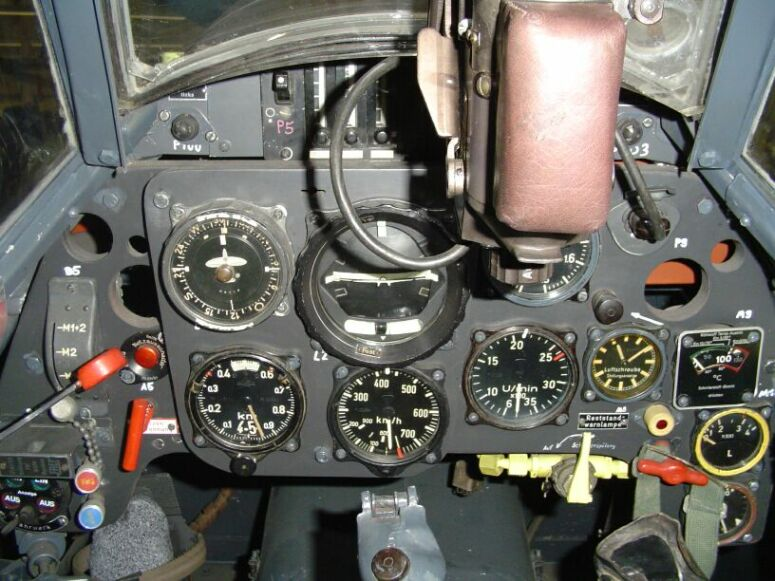
\includegraphics[scale=0.42]{obrazky-figures/G2_dashboard.jpg}
				\caption{Přístrojová deska stíhacího letounu Bf109-G2\protect\footnotemark}\label{historie::vyvojPristroju::kokpitG2}
			\end{center}
		\end{figure}
		\footnotetext{zdroj: \url{http://forum.largescaleplanes.com/index.php?showtopic=8725}}
	
		\begin{figure}[H]
			\begin{center}
				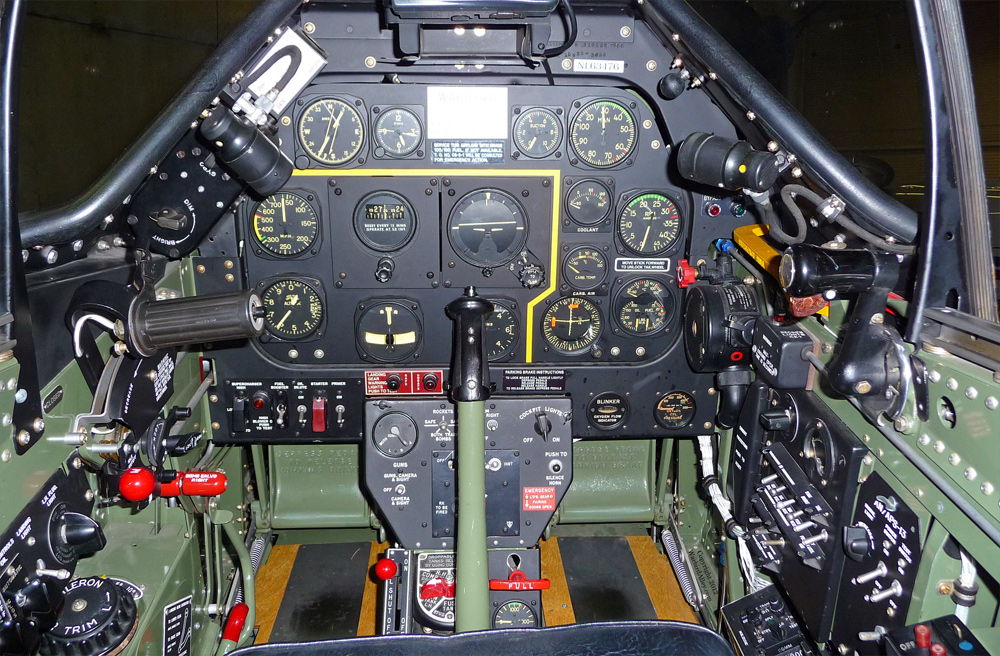
\includegraphics[scale=0.4]{obrazky-figures/P51-cockpit-1000.jpg}
				\caption{Kokpit doprovodného stíhacího letounu P51\protect\footnotemark}\label{historie::vyvojPristroju::kokpitP51}
			\end{center}
		\end{figure}
		\footnotetext{zdroj: \url{http://www.warbirdalley.com/p51.htm}}
		
		
	\section{Vývoj měření výšky a~úvod do této problematiky}
	
		Barometry byly lidstvu známy již od~17. století, tyto bohužel obsahovaly vodu. Aby mohl být tlak vzduchu úspěšně změřen, barometr vyžadoval přibližně 10 metrů vysokou trubici. Avšak italskému matematikovi a~fyzikovi Evangelistovi Torricellimu se podařilo zkrátit délku trubice na 80cm nahrazením vody rtutí, která je cca třináctkrát hustší než voda. I~přes své relativně malé rozměry je tento barometr pořád příliš velký pro masové rozšíření. Za další zmenšení přístroje je zodpovědný francouzský vědec Lucien Vidi, který vynalezl aneroidní barometr, přezdívaný aneroid\cite{history::aneroid}.\par
		Díky této změně se barometr zmenšil na rozumnou velikost a~již se dal použít v~omezeném prostoru letadel. Ve skutečnosti je barometrický výškoměr pouze překalibrovaný aneroid. Bohužel stejně jako ukazatel indikované rychlosti je závislý na mnoha faktorech. Mimo jiné můžeme jmenovat teplotu a~vlhkost vzduchu. Zásadním problémem je, že~barometrický výškoměr už z~principu neukazuje relativní výšku nad terénem, ale~výškud AMSL(height Above Mean Sea Level). Reálně tedy dvě letadla letící podle výškoměru ve výšce 6000 stop několik desítek námořních mil od sebe mohou být v~jiné nadmořské výšce. Na obrázku \ref{historie::vyvojMereniVysky::FL} je názorná ukázka. Zde může čtenáře napadnout, zda se letadla kvůli rozdílným indikovaným hodnotám nesrazí. Barometrické výškoměry sice ukazují nadmořskou výšku špatně, ale~když se letadla přiblíží, tak ukazují stejně špatně a~letadla se tedy minou.\par
		
		\begin{figure}[H]
			\begin{center}
				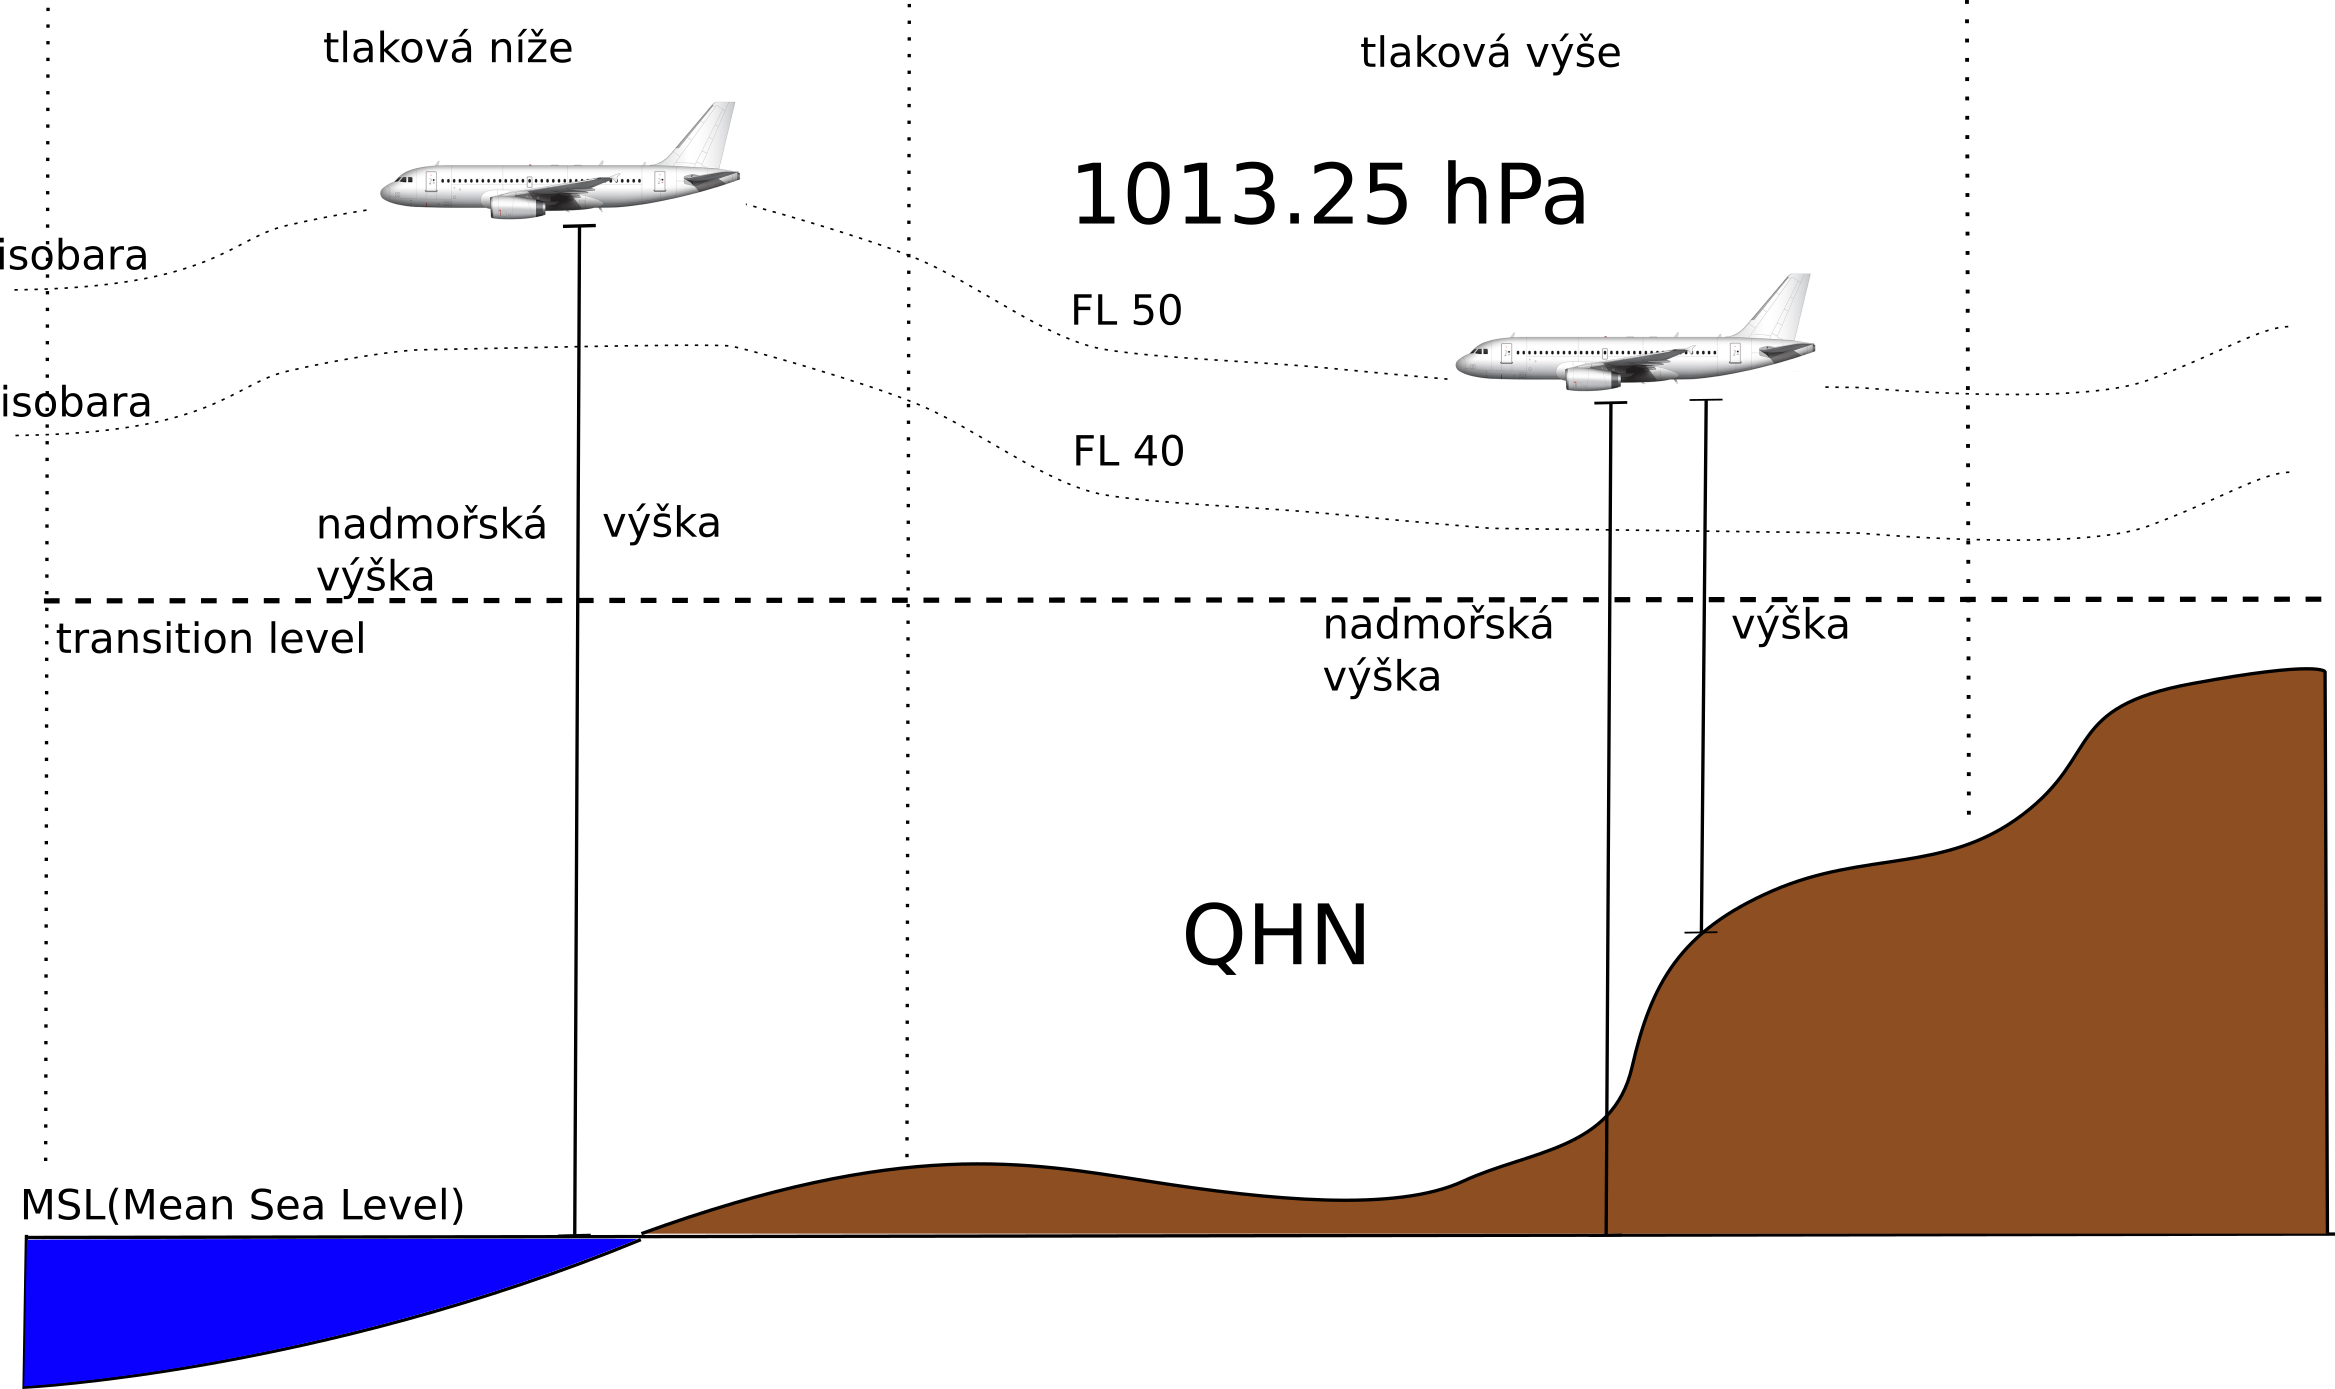
\includegraphics[scale=0.75]{obrazky-figures/flight_level.png}
				\caption{Rozdíl mezi barometrickou(nadmořskou) výškou a~aktuální výškou}\label{historie::vyvojMereniVysky::FL}
			\end{center}
		\end{figure}
				
		Další potíže nastávají s~rozdílnými atmosférickými tlaky mezi počátečním a~cílovým letištěm. Mějme následující situaci: Letadlo letí z~letiště Shiphol v~Amsterdamu, které je tři metry pod hladinou moře, do Himalájí. Zde se v~Tibetu nachází letiště Bangda ve výšce 4334 metrů\cite{bangda}. Rychlou úvahou dojdeme k~závěru, že~ si pilot bude muset dávat pozor v~jaké výšce nad terénem letí a~na jakou výšku bude přistávat. Toto bylo vyřešeno přidáním možnosti kalibrace. Pilot před vzletem nastaví hodnotu QNH, kterou pilotovi sdělí řídící letového provozu, taktéž před přistáním učiní řídící v~cílové oblasti. Na obrázku \ref{historie::vyvojMereniVysky::109Altimeter} můžeme vidět bíle okénko ukazující tlak QNH a~kolečno pro jeho nastavení. Do přechodové hladiny se používá tento výškoměr a~nad touto hladinou pilot letí podle druhého výškoměru, který je pevně nastaven na hodnotu 1013.25 hPa. Toto je pevně zavedený standard pro veškeré civilní lety.\par
		
		\begin{figure}[H]
			\begin{center}
				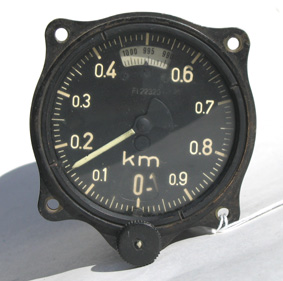
\includegraphics[scale=0.75]{obrazky-figures/109Altimeter.jpg}
				\caption{Výškoměr z~letounu Bf109\protect\footnotemark}\label{historie::vyvojMereniVysky::109Altimeter}
			\end{center}
		\end{figure}
		\footnotetext{zdroj: \url{http://www.warbirdsite.com/Collection.html}}
		
		S~nástupem satelitních technologií se začaly využívat systémy satelitní navigace. Toto upřesnilo navigaci a~již se nemusíme spoléhat pouze na pozemní kontrolu při určovaní pozice letadla. Pomocí systému GPS je schopna posádka určit přesnou pozici na Zemi, rychlost a~azimut během několika sekund aniž by se musela spoléhat na nepřesné pozemní radary.\par 
		
		\paragraph{Existující radarové výškoměry}
		Dalším zdokonalením bylo uvedení radarových výškoměrů. Ty jsou využívány jako hlavní součást GPWS(Ground Proximity Warning System), kde měří absolutní výšku nad terénem. Toto se využívá ve velkých letadlech vážících desítky tun. Našim cílem je vyvinout dostatečně malý, ale~výkonný vestavěný systém, který by radarové výškoměry zpřístupnil i~pro segment lehkých a~ultralehkých letadel.
	
	\section{Vývoj radaru}
		Zrození radaru se datuje do počátku 20. století, kdy~si mocnosti nezávisle na~sobě uvědomily význam této technologie. Mezi lety 1934 a~1939 začaly USA, Velká Británie, Německo, Sovětský svaz, Japonsko, Nizozemsko, Francie a~Itálie nezávisle na sobě vyvíjet systém detekce pomocí radiových vln.\cite{history::radar} Vývoj radaru výrazně pomohl při~bitvě o~Británii, kdy~britové detekovali formující se letadla Luftwaffe nad Francouzským územím, a~tímto umožnil rychlou odezvu Britských pilotů.\par
			
		Během studené války se radary výrazně zdokonalily. Zvětšil se jejich výkon a~zmenšila se jejich velikost. V~současné době se radary houfně využívají k~mírovým účelům, od~sledování počasí přes letectví či~posuny zemské kůry až po mapování.
		
\chapter{Použité technologie a teorie přistání}
	
	\section{Radary a~jejich dělení}\label{uvod::radary}
		Radar (\textbf{RA}dio \textbf{D}etection \textbf{A}nd \textbf{R}anging) je systém pro detekci objektů, u~kterých~je pomocí rádiových vln schopen určit vzdálenost, azimut a~rychlost sledovaných objektů. Využití radarů je široké, od~mapování terénu, detekce osob přes měření rychlosti vozidel a~využití v~civilním letectví až~po~vojenské účely.	
			
	\paragraph{Klasifikace radarů}
			Radary se dělí podle typu vysílání a~podle použití\cite{radarClasification}. Základní dělení je: 
			\begin{itemize}
				\item \textbf{Primární radar}	-	Slouží k~zobrazování objektů ve vzdušném prostoru. Vysílač vysílá vysokofrekvenční signál a~přijímač zachytává ozvěnu vysílaného signálu. Na příslušném místě na obrazovce posléze vykreslí, v~profesním slangu řečeno, knedlík, podle pozice objektu ve vzdušném prostoru vůči radarové stanici.
					
				\item \textbf{Sekundární radar}	-	Slouží k~přenosu informací mezi radarovou stanicí a~letadlem. Aby toto spojení fungovalo, musí mít cílový objekt zapnutý transpondér v~příslušném módu, který~po přijetí signálu zpracuje dotaz a~odpoví požadovanými informacemi např. výška, rychlost, souřadnice GPS a~kurz. 
			\end{itemize}
			
			Primární radary se dále dělí na:
			\begin{itemize}
				\item \textbf{Pulsní}	-	Tomuto typu radarů postačuje pouze jedna anténa a~to z~toho důvodu, že~se radar periodicky přepíná mezi vysílacím režimem a~přijímacím režimem. Z~tohoto pramení nevýhoda tohoto typu radarů: minimální a~bez modulací i~maximální dosah. Minimální dosah radaru je určen rychlostí přepínaní mezi jednotlivými režimy. Pokud se vrátí ozvěna dříve, než~se radar přepne do~přijímacího režimu, radar objekt nedetekuje a~informace je ztracena. Obdobně to funguje i~u~maximálního dosahu. Radar musí zachytit ozvěnu před vysláním dalšího impulsu.
				
				\item \textbf{Kontinuálně vysílající}	-	Radary tohoto typu vysílají nepřerušovaně a~zároveň nepřerušovaně zpracovávají přijatou ozvěnu, proto potřebují jak vysílací, tak přijímací anténu. Tyto radary se dělí na:
					
					\begin{itemize}
						\item Modulované - Tyto radary využívají frekvenční modulace signálu, díky které jsme schopni vypočítat vzdálenost z~ozvěny vysílaného signálu. Toto je typ radaru, kterým bude vybaveno naše zařízení.
						
						\item Nemodulované - Tyto radary vysílají konstantní signál, který~umožňuje pouze určení rychlosti zachycených objektů.
					\end{itemize}
					
					U FM-CW\footnotemark\footnotetext{Frequency-Modulated Continuous-Wave} radarů je oproti pulsním radarům měření vzdálenosti podstatně komplikovanější. TODO zeptat se vedoucího co tu chce.
			\end{itemize}
		
		\section{Vestavěné systémy}
			Jelikož náš systém má jediný účel, a~to zjistit výšku letadla nad přistávací dráhou, využívat víceúčelová zařízení je pro~nás zbytečně robustní a~neforemné. Potřebujeme jednoduché, rychlé a~elegantní zařízení, které~bude plnit pouze jediný úkol. Zde přicházejí do hry vestavěné systémy.
			
			\begin{definice}
				Vestavěné systémy VS jsou systémy, ve~kterých~je zpracování dat vestavěno/vloženo do~většího systému a~ve~kterém není zpracování dat viditelné uživateli prostřednictvím např. PC počítače. Anglicky se vestavěné systémy označují jako \textbf{embedded system}\cite{impSkripta}.
			\end{definice}
			
			Vestavěné zařízení je jednoduchý a~elegantní způsob řešení jednotvárných algoritmických úloh. Naše úloha musí být vykonávána v~reálném čase, tzn. máme určenou dobu odezvy a~tu musíme splnit. Nutnost mít co nejnižší odezvu určuje nároky na~zvolené zařízení. Na tomto zařízení poběží pouze jediná aplikace. To nám umožňuje optimalizovat aplikaci na~míru systému pro dosažení co~největšího výkonu.
			Bohužel optimalizace aplikace není vše. Aby se algoritmus vykonával co~nejrychleji, musíme pro ni~zvolit odpovídající zařízení. Pro náš systém potřebujeme zajistit dostatečně rychlé vzorkování abychom zabránili aliasingu. Toto je nejlepší řešit na~hardwaru, jelikož rychlost zpracování bude vyšší a~budeme schopni zaručit splnění podmínky Nyquistova teorému, kdy~vzorkovací frekvence musí být alespoň dvakrát větší než~maximální frekvence signálu: \[f_v > 2f_{max}\]
			
			Pro tuto úlohu se hodí programovatelné hradlové pole FPGA. Toto pole bude vzorkovat signál s~dostatečnou frekvencí a~po sběrnici jednotlivé vzorky posílat dále do procesoru pro zpracování.\par
			
			\paragraph{Xilinx Zynq}
				Po určení požadavků na~hardware v~úvahu připadají zařízení od~výrobce programovatelných hradlových polí Xilinx. Konkrétně rodina procesorů Zynq, která~kombinuje FPGA s~procesorovým jádrem ARM Cortex.
				Jak již bylo zníněno výše, FPGA navzorkuje signál a~pošle jej k~dalšímu zpracování přez AXI porty jádru procesoru ARM, na kterém poběží odlehčená verze Linuxu. Na tomto operačním systému poběží aplikace provádějící potřebné výpočty a~bude posílat výsledek na výstup.
				
				\begin{figure}[h]
					\begin{center}
						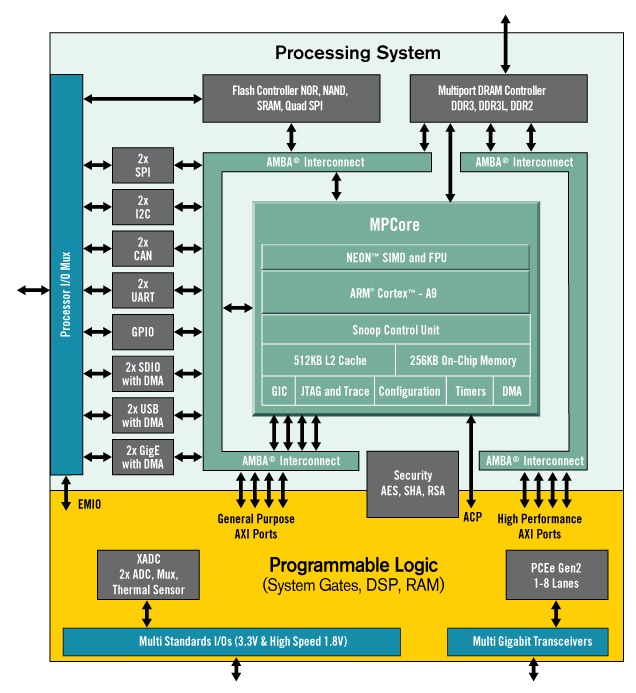
\includegraphics[scale=0.6]{obrazky-figures/zynq-mp-core-single.png}
						\caption{Architektura procesoru Zynq-7000\protect\footnotemark}
						\label{teorie::embedded::zynq}
					\end{center}
				\end{figure}
				\footnotetext{zdroj: \url{https://www.xilinx.com/products/silicon-devices/soc/zynq-7000.html}}
			
			\paragraph{Řídící modul}
				Řídící modul obsahující výše zmíněný procesor je dodán společností CAMEA s.r.o. Modul obsahuje vstupně výstupní porty , které~můžeme využít v~náš prospěch. Jako výstupní porty můžeme využít USB sběrnici s~přímým přístupen do paměti, GPIO porty nebo Serial Peripheral Interface. 
				\begin{itemize}
					\item USB můžeme využít pro přenos přesných informací obrazovou formou na displej, kde zobrazujeme výšku, případně využít externí USB zvukovou kartu pro generování zvukových signálů. 
					
					\item Pomocí GPIO portů, případně rozhraní SPI, můžeme ovládat panel s~LE Diodami, který~barevnými LED seřazenými vertikálně. Tento panel bude mít diody vyzařující světlo od~zeleného spektra, přes žlutou, oranžovou a~sytě červenou, kdy~bude začínat fáze dosednutí.
					
					\item Zvuková komunikace může probíhat generováním tónů a~odesílání konektorem typu 3.5mm Jack. Bude se generovat stále stejný tón konstantní délky, přičemž zkracující se perioda bude signalizovat snižující se výšku. Pokud bude letadlo těsně nad zemí, bude se generovat tón bez přerušení.
				\end{itemize}
			
			\paragraph{Kalibrace modulu}
				Další částí naší úlohy je nutnost kalibrace zařízení, jelikož každé letadlo může mít tento modul umístěno v~jiné výšce nad zemí. Kalibrace může být statická - v~kódu bude přičtena konstanta, nebo dynamická, kdy~se před startem modul zkalibruje. Statická kalibrace má výhodu jednoduššího chování modulu a~bude vyžadovat o~jeden ovládací prvek méně, avšak bude nutno zasahovat do zdrojových kódů při instalaci na jiné letadlo. Dynamická kalibrace, na rozdíl od~statické, má nevýhodu složitějšího řídícího programu, ale~bude možno mít jeden program pro všechny typy letadel. Přidaný ovládací prvek nebude téměř znát. V~tomto případě se autor přiklání k~dynamické kalibraci.
				
			\paragraph{Ovládací panel}
				Nutnost kalibrace nás přivádí k~ovládacímu panelu modulu. Přístroj je třeba nějak zapnout, toto bude první přepínač. Dále vyvstává otázka nutnosti mít vždy zapnutou zvukovou signalizaci. Jelikož bude využití tohoto výškoměru při vzletu mizivé, bude dobré, když~bude mít pilot možnost vypnout zvukovou indikaci, která~v~situaci, kdy~ji není potřeba může působit rušivě. Proto může být přítomen přepínač ovládající tuto funkci. Jako třetí kontrolní prvek zvolíme tlačítko spouštějící kalibraci přístroje na referenční hodnotu země. Je nutné, abychom zabránili kalibraci výškoměru ve vzduchu, proto by mělo toto tlačítko být překryté víčkem. V~případě, že~bude koncipováno jako ovládací prvek na dotykovém displeji, za~pohybu letadla by mělo být deaktivované.
				
	\section{Teorie přistání}
		Letadlo, které vzlétne, musí zpět na zem. Ideálně rozumným a~hlavně bezpečným způsobem. Není žádoucí, aby se jak letadlu, ale~hlavně pasažérům cokoliv přihodilo. Způsobilo by to nejen finanční ztráty. Proto je kladen velký důraz na výuku a~správné naučení přistávání.  

		\begin{figure}[H]
			\begin{center}
				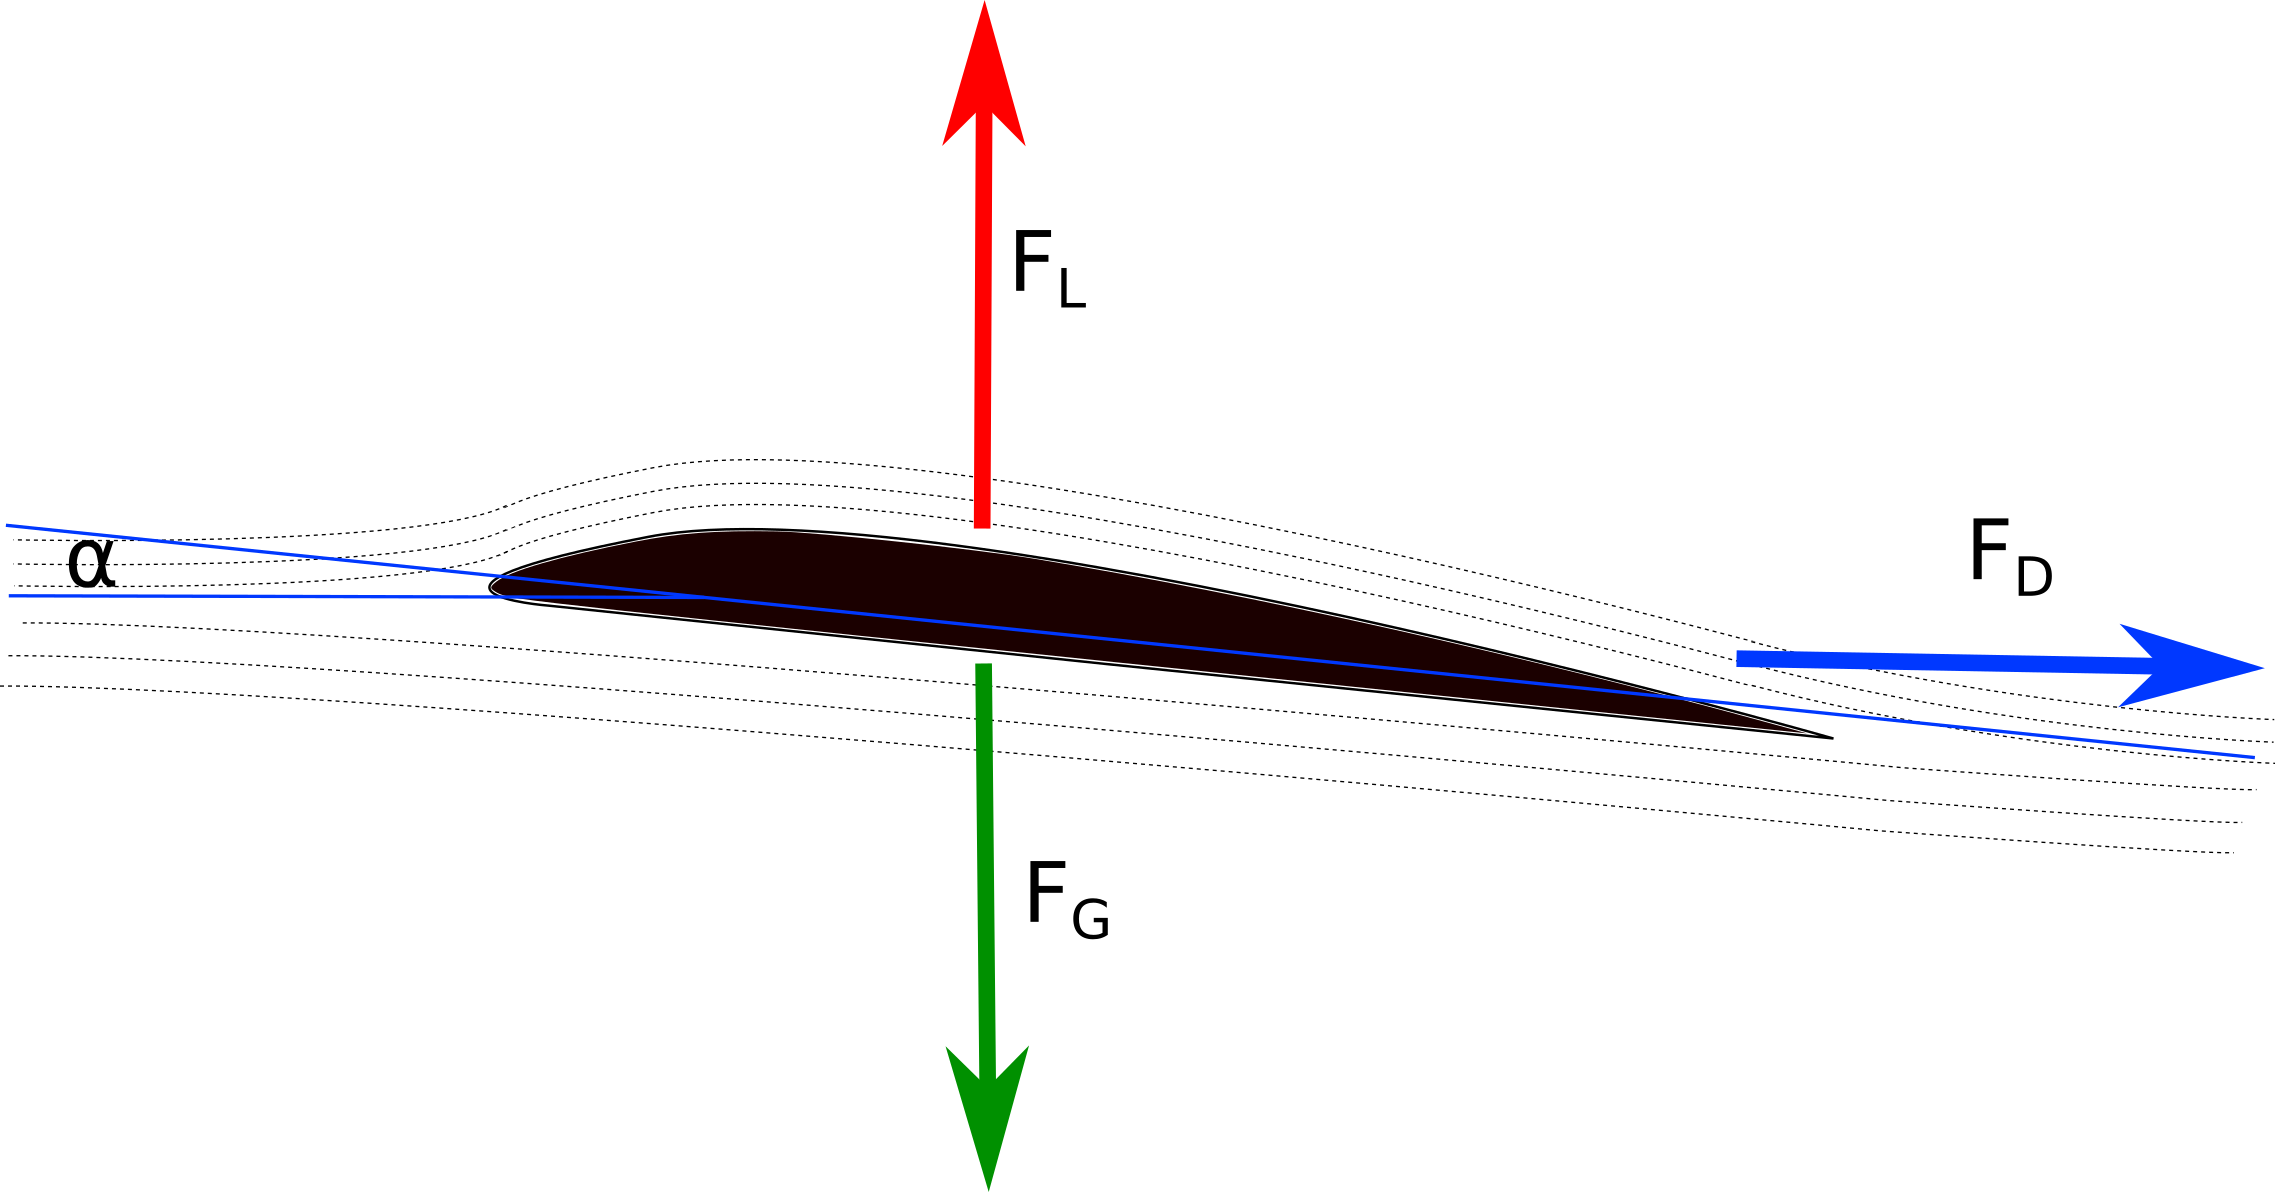
\includegraphics[scale=0.7]{obrazky-figures/angle_of_attack.png}
				\caption{Proudění vzduchu podél křídla.}
				\label{teorie::pristani::angle_of_attack}
			\end{center}
		\end{figure}
		
		Když se blíže podíváme na přistání, je to doslova řízený pád. Na obrázku \ref{teorie::pristani::angle_of_attack} můžeme vidět příklad proudění vzduchu podél křídla konvenční konstrukce. $F_L$ značí vztlakovou sílu(lift), $F_G$ značí gravitační sílu(gravity), $F_D$ značí odpor vzduchu(drag) a~$\alpha$ značí úhel náběhu. Díky tomuto tvaru nad křídlem proudí vzduch rychleji než pod křídlem, podle Bernoulliho rovnice to znamená, že~nad křídlem má vzduch menší hustotu než pod a~dochází ke vzniku vztlaku. Čím větší je úhel náběhu, tím větší je vztlak a~zároveň se zvětšuje odpor vzduchu. Toto platí pouze za podmínky, kdy je úhel náběhu menší než je jeho kritická hodnota. Od této kritické hodnoty, kterou má každý tvar křídla jinou, dochází ke snižování generovaného vztlaku až k~nule ale~odpor vzduchu stále stoupá. To znamená, že~letadlo ztrácí rychlost a~výšku. Na pilotovi je, tento řízený pád udržel v~rozumné míře a~nepropadl se do nekontrolovatelného pádu, jelikož při přistání není mnoho prostoru pro znovuzískání kontroly nad letadlem.\par
		Přistání lze rozdělit do několika fází\cite{landingPhases}.
		
		\begin{enumerate}
			\item STAR(\textbf{S}tandard \textbf{T}erminal \textbf{A}rrival \textbf{R}oute) - Po opuštění letové trasy letadlo provede prvotní přiblížení po trase určené v~letecké informační příručce(AIP). 
			
			\item ILS Přiblížení (\textbf{I}nstrument \textbf{L}anding \textbf{S}ystem \textbf{A}pproach) - Po ukončení STARu pilot na základě uděleného povolení provede přiblížení pomocí přístrojů, které ho přesně navádějí na dráhu. V~této fází si pilot připraví letadlo do přistávací konfigurace.
		
			\item Závěrečné přiblížení (Final approach) - Během této fáze pilot musí udržovat přibližovací rychlost danou výrobcem letadla a~letět po kurzu osy dráhy pod sklonem určeným přibližovacími pravidly(glidepath). Zde do hry vstupuje naše zařízení, které bude pilotovi oznamovat výšku stroje nad terénem.
					
			\item Výdrž - Když se pilot přibližuje k~dráze, musí přitáhnout knipl, tím zvýší úhel náběhu a~jak jsme si již vysvětlili výše, způsobí zpomalení stroje. Pilotovým úkolem v~této fázi letu je s~vypnutým motorem udržovat letadlo ve vodorovném letu těsně nad dráhou, na kterou~pak díky ztrátě vztlaku dosedne. Je důležité, aby letadlo bylo těsně nad dráhou, čím výše se v~okamžiku ztráty vztlaku letadlo nachází, tím tvrdší přistání může čekat. A~tím větší škody mohou vzniknout.
					
			\item Dosednutí a~rolování (Touchdown and taxi) - Po dosednutí pilot zpomalí letadlo na požadovanou rychlost pro rolování a~roluje na místo určené řídícím letového provozu. 
		\end{enumerate}
				
\chapter{Návrh řešení}\label{navrhReseni}
	Nejdříve si musíme uvědomit, co je našim cílem, analyzovat zadání a~podle něj si pak navrhnout vhodné řešení. Vhodným se rozumí jednoduché, efektivní a~rozšířitelné pro další využití.\par
	
	\begin{figure}[H]
		\begin{center}
			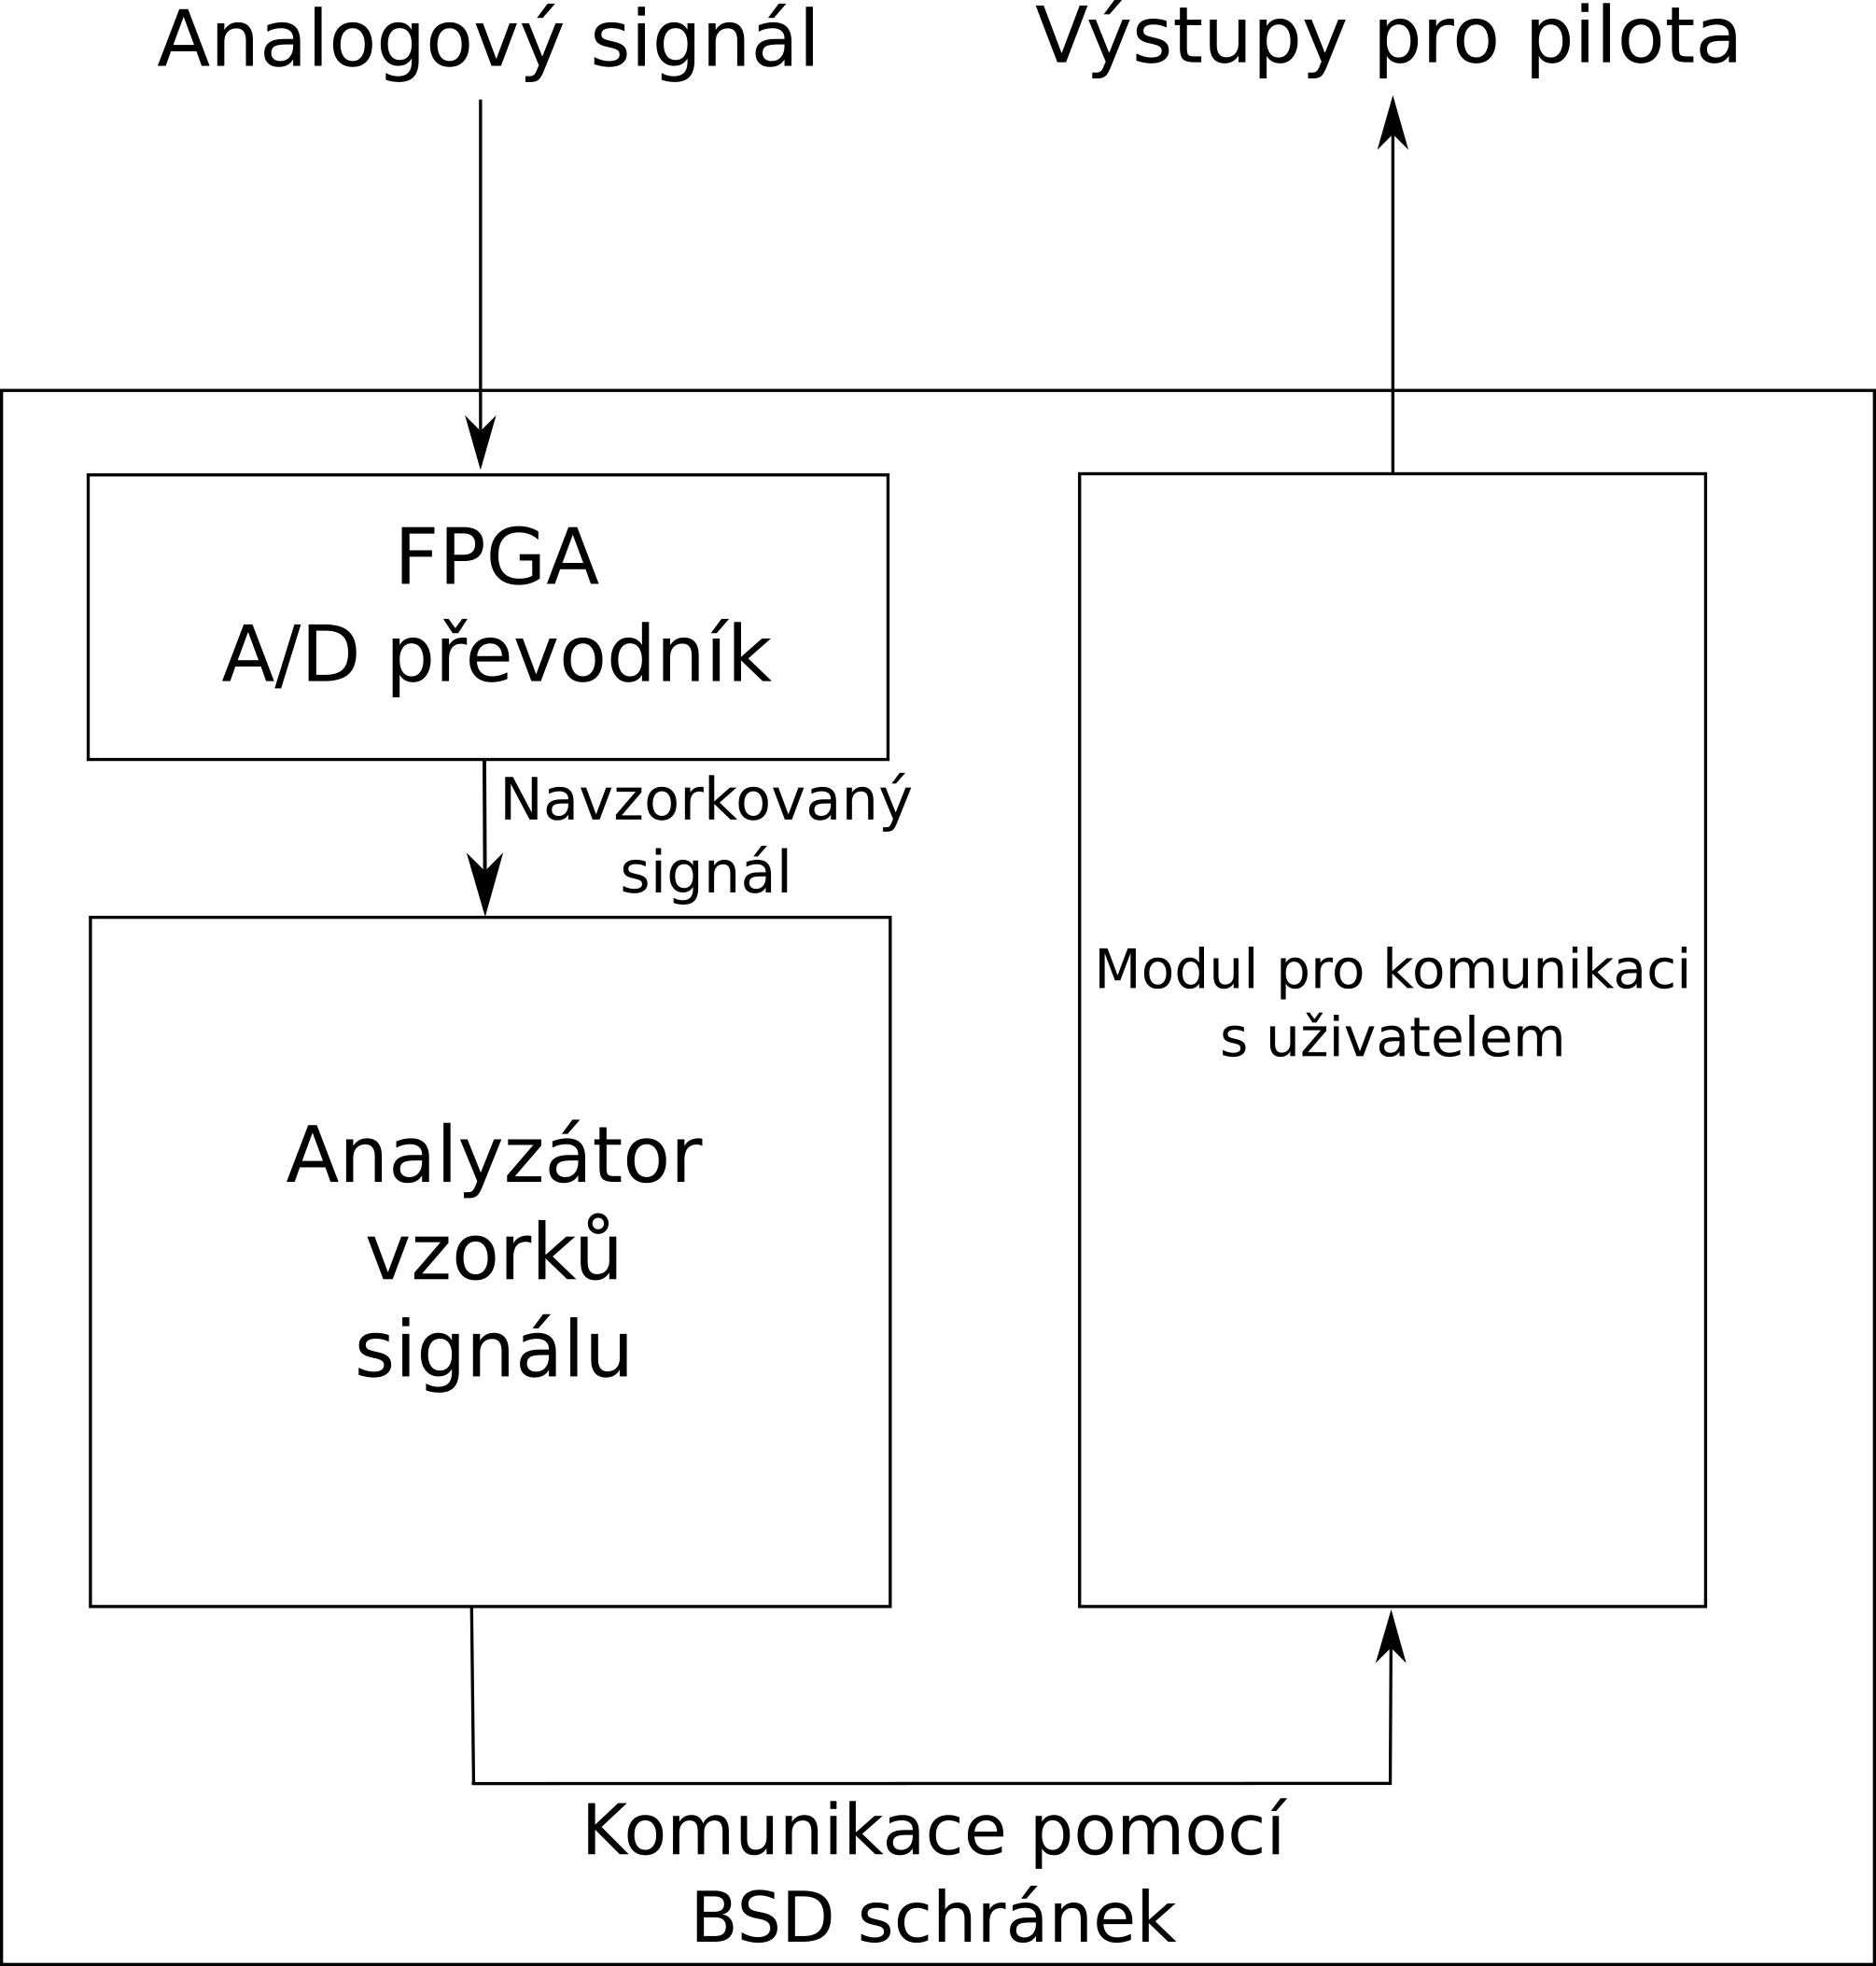
\includegraphics[scale=0.7]{obrazky-figures/navrh_obecne.png}
			\caption{Moduly}
			\label{navrh::moduly}
		\end{center}
	\end{figure}
	
	Kvůli omezenému prostoru naše zařízení byt malé, kvůli zachování aktuálnosti předané informace rychlé, kvůli spotřebě elektrické energie energeticky nenáročné a~kvůli podmínkám, ve kterých bude pracovat odolné vůči vnějším vlivům. Naštěstí nároky na rychlost zpracování nejsou příliš přísné. Průměrný člověk má reakční dobu přibližně sekundu, v~závislosti na tréningu a~požadované reakci. Zároveň ale~platí, že~čím rychlejší náš systém bude, tím přesnější informace budeme schopni dodávat pilotovi. Předané informace musí být ve vhodném formátu pro rychlou a~bezchybnou interpretaci pilotem, aniž by působily rušivě a~odváděly pozornost.
	
	\section{Platforma}\label{navrhReseni::platforma}
		Jak již bylo zmíněno v~úvodu této kapitoly, potřebujeme malé, ale~rychlé zařízení, které bude v~reálném čase poskytovat údaje o~aktuální výšce. V~našem případě, vzhledem k~reakční době člověka okolo sekundy, bude stačit, když systém stihne spočítat výsledek a~předat jej pilotovi do $\sim$250ms.\par
		
		Kvůli nárokům na velikost a spotřebu můžeme vyřadit objemné osobní počítače s~architekturou x86 případně AMD64 a~spíše se ponořit do~oblasti vestavěných systémů. V~současnosti trh nabízí dostatečně výkonné a~zároveň dostatečně kompaktní zařízení, která~jsou pro náš účel vhodná. Jako možný kandidát se jeví mikropočítač Raspberry Pi, který už je dostatečně výkonný a~zároveň malý aby mohl splnit požadavky naši úlohu. Bohužel, kvůli konektivitě je tato platforma nevhodná. Jako další se nabízí Arduino. Tato platforma nabízí solidní výkon za rozumné peníze. Bohužel tento výkon nedostačuje našim potřebám a~hodí se spíše do nově rozvíjejícího se oboru Internet of Things. Vhodnější alternativa k~tomuto řešení se jeví procesor rodiny Zynq od~výrobce Xilinx, který je určen přesně pro naše potřeby, a~díky integrovaným programovatelným hradlovým polím FPGA výrazně urychluje zpracování ozvěny signálu byť už jen pouhým vzorkováním daného signálu. Přístroj s~procesorem dodala společnost CAMEA s.r.o. Na tomto procesoru bude spuštěn operační systém OpenSUSE, který bude obsluhovat naši aplikaci.
		
	\section{Hardware}
		Radarový transciever, se~kterým~pravděpodobně budeme v~této práci pracovat je IVS-948 firmy InnoSenT dodaný firmou CAMEA s.r.o. Jedná se o~kontinuálně vysílající a~přijímající radar s~frekvenční modulací. Díky frekvenční modulaci vysílaného signálu jsme schopni změřit nejenom rychlost překážky, ale~i~jeho vzdálenost, což je přesně to, co pro naše účely potřebujeme.
	
	\paragraph{Výstupní zařízení}
		Náš systém musí pilotovi nějak interpretovat sesbíraná data, jinak by byl zbytečný. Způsob komunikace musí být tak detailní, aby dokázal předat informace o~výšce nad~zemí a~zároveň dostatečně jednoduchý, aby pilot mohl data ze~systému zpracovat rychle a~efektivně aniž by výstupní zařízení odvádělo pozornost od~právě prováděných úkonů. Jedna z~možností je použití zvukových signálů, druhá je zobrazování aktuálních informací na přístrojové desce letounu. Zde si musíme položit otázku, jaký z~těchto způsobů zvolíme. Zobrazení dat na přístrojové desce nabízí možnost jejich nejpřesnější interpretace, bohužel bude odvádět pozornost pilota a~zvyšuje se riziko nehody. Jako další nevýhodu autor vidí zbytečně zabraný prostor, jehož přidaná hodnota po osazení přístrojem pro zobrazovaní dat není dostatečná pro naše použití. 
			
	\paragraph{Vstupní zařízení}		
		Pilot musí být schopen zařízení také ovládat. Proto se musíme zamyslet nad možnými ovládacími prvky.
		Zařízení budeme muset nějak zapnout a kalibrovat. Máme dvě možnosti. Buď se zařízení bude zapínat a vypínat automaticky zároveň s motorem, nebo jej bude moci pilot ovládat. Autor se přiklání k možnosti ovládání pilotem, jelikož v pozdějších fázích výuky může být asistence našeho systému nežádoucí. Přesně si to určí až zákazník.\par
		Zákazník jistě bude chtít modul také kalibrovat. Zde si musíme uvědomit, že kalibrace se může úspěšně provést pouze, když letadlo stojí na zemi v klidu. Dochází totiž k nastavení referenční hodnoty výšky zařízení nad dráhou a není žádoucí aby se kalibrace prováděla ve vzduchu. Možné následky jsme si již uváděli. Spuštění musí být jednoduché a zároveň k němu nesmí dojít náhodou. Proto se nabízí možnost krytého tlačítka. Inspirovat se můžeme u stíhacích letounů, kdy při odklopení krytky dochází k odjištění zbraní. Finální podobu si opět určí zákazník.
	
	\section{Software}\label{navrhReseni::software}
		Zde si musíme připomenout, že~našim úkolem není zpracování signálu. Program pro obsluhu generování informací pro pilota musí být rychlý, spolehlivý a relativně nenáročný na výpočetní výkon.
		
		\paragraph{Komunikace}
		Moduly mezi sebou musí komunikovat, přičemž nesmí docházet ke ztrátě dat, zpoždění nebo pádu aplikace. Nejdříve se musíme zamyslet nad vhodným způsobem komunikace.\par 
		Jako první se podívejme na komunikační rozhraní CORBA(\textbf{C}ommon \textbf{O}bject \textbf{R}equest \textbf{B}roker \textbf{A}rchitecture). Toto rozhraní poskytuje dobrý komunikační kanál v~případě, že je třeba komunikovat mezi procesy na jednom stroji případně mezi procesy na více strojích. Aby CORBA fungovala, potřebuje spuštěný CORBA Name Server. Bohužel tato aplikace by zabírala potřebné prostředky a nemusel by zbýt výkon pro nutné věci. Další důvod pro zamítnutí tohoto řešení je jeho robustnost nevhodná pro vestavěné systémy.\par
		Jako další možnost se jeví využití sdílené paměti. Ta umožňuje velice rychlé předávání dat za nízkého úbytku výkonu. Toto řešení ovšem vyžaduje zabezpečovací mechanismus pro zachování konzistence. Kvůli složitosti tohoto mechanismu se od řešení pomocí sdílené paměti odkloníme a spíše se přikloníme k~modelu klient-server implementovaným pomocí BSD schránek. BSD schránky poskytují již hotovou implementaci komunikace, které je dostatečně rychlá a nezabírá příliš mnoho systémových prostředků, toto je pro naše účely ideální.\par
		Nyní se musíme rozhodnout zda použijeme spojovanou či nespojovanou službu. U~spojované služby nehrozí ztráty paketů, jelikož se v~případě jejich nedoručení posílají znovu. Bohužel toto si nemůžeme dovolit, jelikož tato informace již nebude aktuální. Na rozdíl od spojované služby TCP, nespojovaná služba UDP sice nezajišťuje opětovné poslání paketu, ale zaručí nám, že odesílaná data budou aktuální i v~případě, že se nějaký paket ztratí. Tato ztráta nás vzhledem k~počtu odeslaných paketů nijak neomezí. 

		\paragraph{Architektura modulu}
		Vzhledem k~modelu klient-server musíme zabezpečit paralelní příjímání zpráv a následné vykonání události na základě přijaté zprávy. Kvůli tomuto požadavku nemůžeme využít přímé jedno vláknové zpracování, jelikož obsluha hardware je blokující a docházelo by ke zpoždění, které by akumulací starých paketů vyústilo v~neaktuální až nebezpečné informace. Paket zpožděný o~půl sekundy může mít katastrofální následky. Uveďme příklad. Je léto, slunné počasí a ve stínu je teplota 37 stupňů Celsia. Pilot provádí přiblížení před přistáním na betonové, případně asfaltové dráze. Vzhledem k~rozdílným teplotám vzduchu nad trávou a betonem, případně asfaltem, může při příletu nad dráhu dojít k~prudkému propadu letadla kvůli rozdílným hustotám teplého a studenějšího vzduchu. Tyto propady bývají rychlé a je nutné na ně rychle reagovat a nezmatkovat. Při špatné reakci může dojít k~poškození stroje v~tom lepším případě, a k zranění posádky a pasažérů v~tom horším případě. Ani jedna možnost není žádoucí, proto potřebujeme pracovat pouze s~aktuálními informacemi. V~případě blokujících operací, by mohlo dojít k značnému zpoždění a tedy i škodám. Proto přistoupíme k více vláknovému řešení.\par
		Při práci s více vlákny si musíme dávat pozor na zabezpečení komunikace a musíme zachovat konzistenci dat. Data se předávají mezi vlákny pomocí fronty. Aby bylo jasné, kdo k ní může přistupovat, musí být vhodně zabezpečena a tudíž využijeme mutexy. Jedno vlákno ve bude ve smyčce přijímat zprávy a vkládat je do fronty. Druhé vlákno je z fronty vyjme a provede náležité operace.\par
		
	\section{Komunikační protokol}\label{navrhReseni::protokol}	
		Aby byly dva moduly schopny komunikovat nějakým rozumným způsobem, potřebujeme komunikační protokol.
		U návrhu komunikačního protokolu je třeba zjistit co přesně potřebujeme a pozastavit se nad možnými rozšířeními do budoucna. Mohlo by se zdát, že jedinou potřebnou informací je výška letadla nad terénem. Bohužel tomu tak není. Ano, výška nad terénem je nejdůležitější přenášená informace, ale sama o sobě je nám k ničemu. S danou výškou potřebujeme přenést i časovou informaci, kdy byla výška odeslána abychom mohli zajistit práci pouze s aktuálními informacemi, jak již bylo zmíněno výše. Nyní se ovšem musíme zamyslet, jakým směrem se vývoj zařízení bude ubírat. Tato práce není pouze pro uspokojení akademiků, ale v jejím závěru a v následném vývoji má vzniknout konkurenceschopný výrobek pro trh. Proto můžeme předpokládat výrazný a rychlý vývoj. Pravděpodobně v některé následující iteraci vývoje dojde k rozšíření o informace, v jakém stavu se radar nachází. Jako dobrý krok se jeví také přidání několika bajtů pro zatím neznámé účely.\par
		Finální verze protokolu bude obsahovat příznaky pro přenos stavových informací o velikosti jednoho bajtu a výšku nad terénem, která bude v datovém typu \texttt{double}, jeho velikost se bude lišit podle platformy, na které budou programy spuštěny. Nesmíme zapomenout na časové razítko v mikrosekundách pro identifikaci neaktuálních zpráv, rezervovaný prostor o velikosti osmi bajtů a nakonec ukončující bajt nastaven na nulu. Výsledek můžeme vidět na obrázku \ref{navrh::protokol}
		
		\begin{figure}[H]
			\begin{center}
				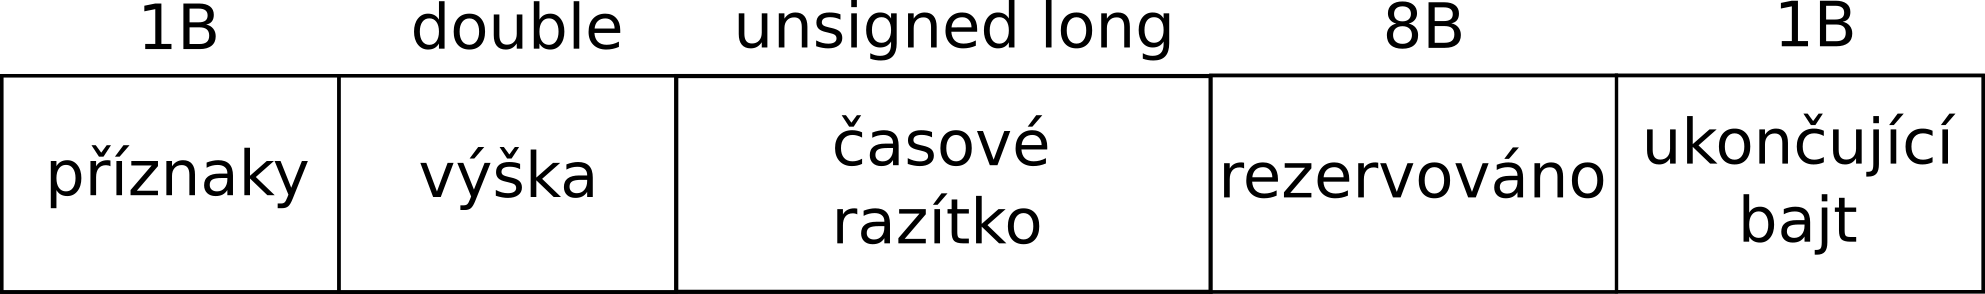
\includegraphics[scale=0.7]{obrazky-figures/protokol.png}
				\caption{Komunikační protokol včetně velikostí jednotlivých částí}
				\label{navrh::protokol}
			\end{center}
		\end{figure}
		

		
		
	\section{Umístění na letadle}\label{navrhReseni::umisteniNaLetadle}
		Nyní se zamysleme nad možnostmi umístění zařízení na letadle. Zařízení musí být na~letadle umístěno tak, ať~je šance poškození přístroje při tvrdším přistání minimální, zároveň musí být měření konzistentní a musí být chráněno i proti povětrnostním podmínkám. Toto vylučuje umístění přístroje na~konci křídel. Může dojít k~odření křídla o~zem při přílišném naklonění, navíc bude muset být provedena velká korekce výšky a~může dojít k~změnám detekované výšky při náklonech letadla, taky dojde k~narušení aerodynamiky křídla, kdy letadlo bude mít tendence stáčet se za křídlem, na kterém se zařízení nachází. Ideální by bylo umístit senzor na pneumatiky jednoho z~kol hlavního podvozku, bohužel velice rychle zjistíme, že~je to nevhodné řešení z~důvodů jednorázového použití radaru. Jako další vhodné možnosti se jeví umístění:
		\begin{itemize}
			\item s odsazením na~nohu podvozku za předpokladu, že~se na~ni zařízení vejde(v případě zatažitelného podvozku). Při umístění na~pevný podvozek je třeba zamezit možnosti vzniku poškození následkem tvrdého přistání a špatného počasí. 
			
			\begin{figure}[H]
				\begin{center}
					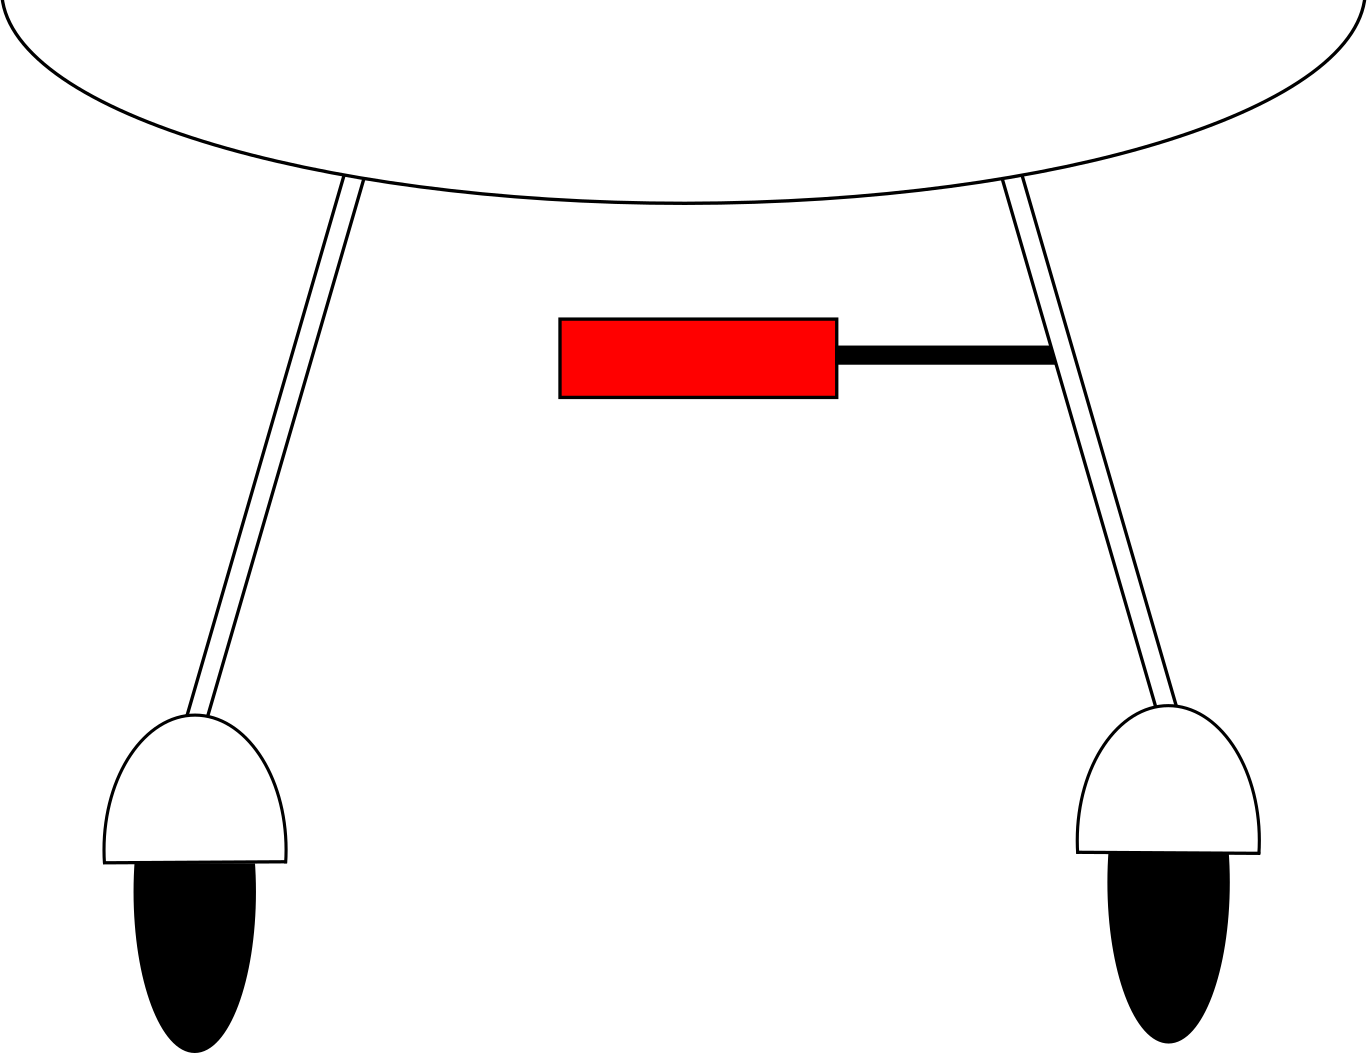
\includegraphics[scale=0.5]{obrazky-figures/umisteni_na_podvozku.png}
					\caption{Montáž na podvozku}
					\label{navrh::umisteni_podvozek}
				\end{center}
			\end{figure}
			
			\item na~spodní část kořene křídla, kde~nebude moment síly způsobující rotaci letadla ve~vodorovné ose tak velký, jako na konci křídla. Otřesy, které~bude muset zařízení snášet nebudou tak velké jako na noze hlavního podvozku. Stále je třeba myslet na ochranu proti špatnému počasí. Další nevýhoda je nutnost vrtání do trupu či křídla kvůli ukotvení. Bohužel zde zůstává nutnost korekce podle výšky kořene letadla nad~rovinou podvozku.
			
			\begin{figure}[H]
				\begin{center}
					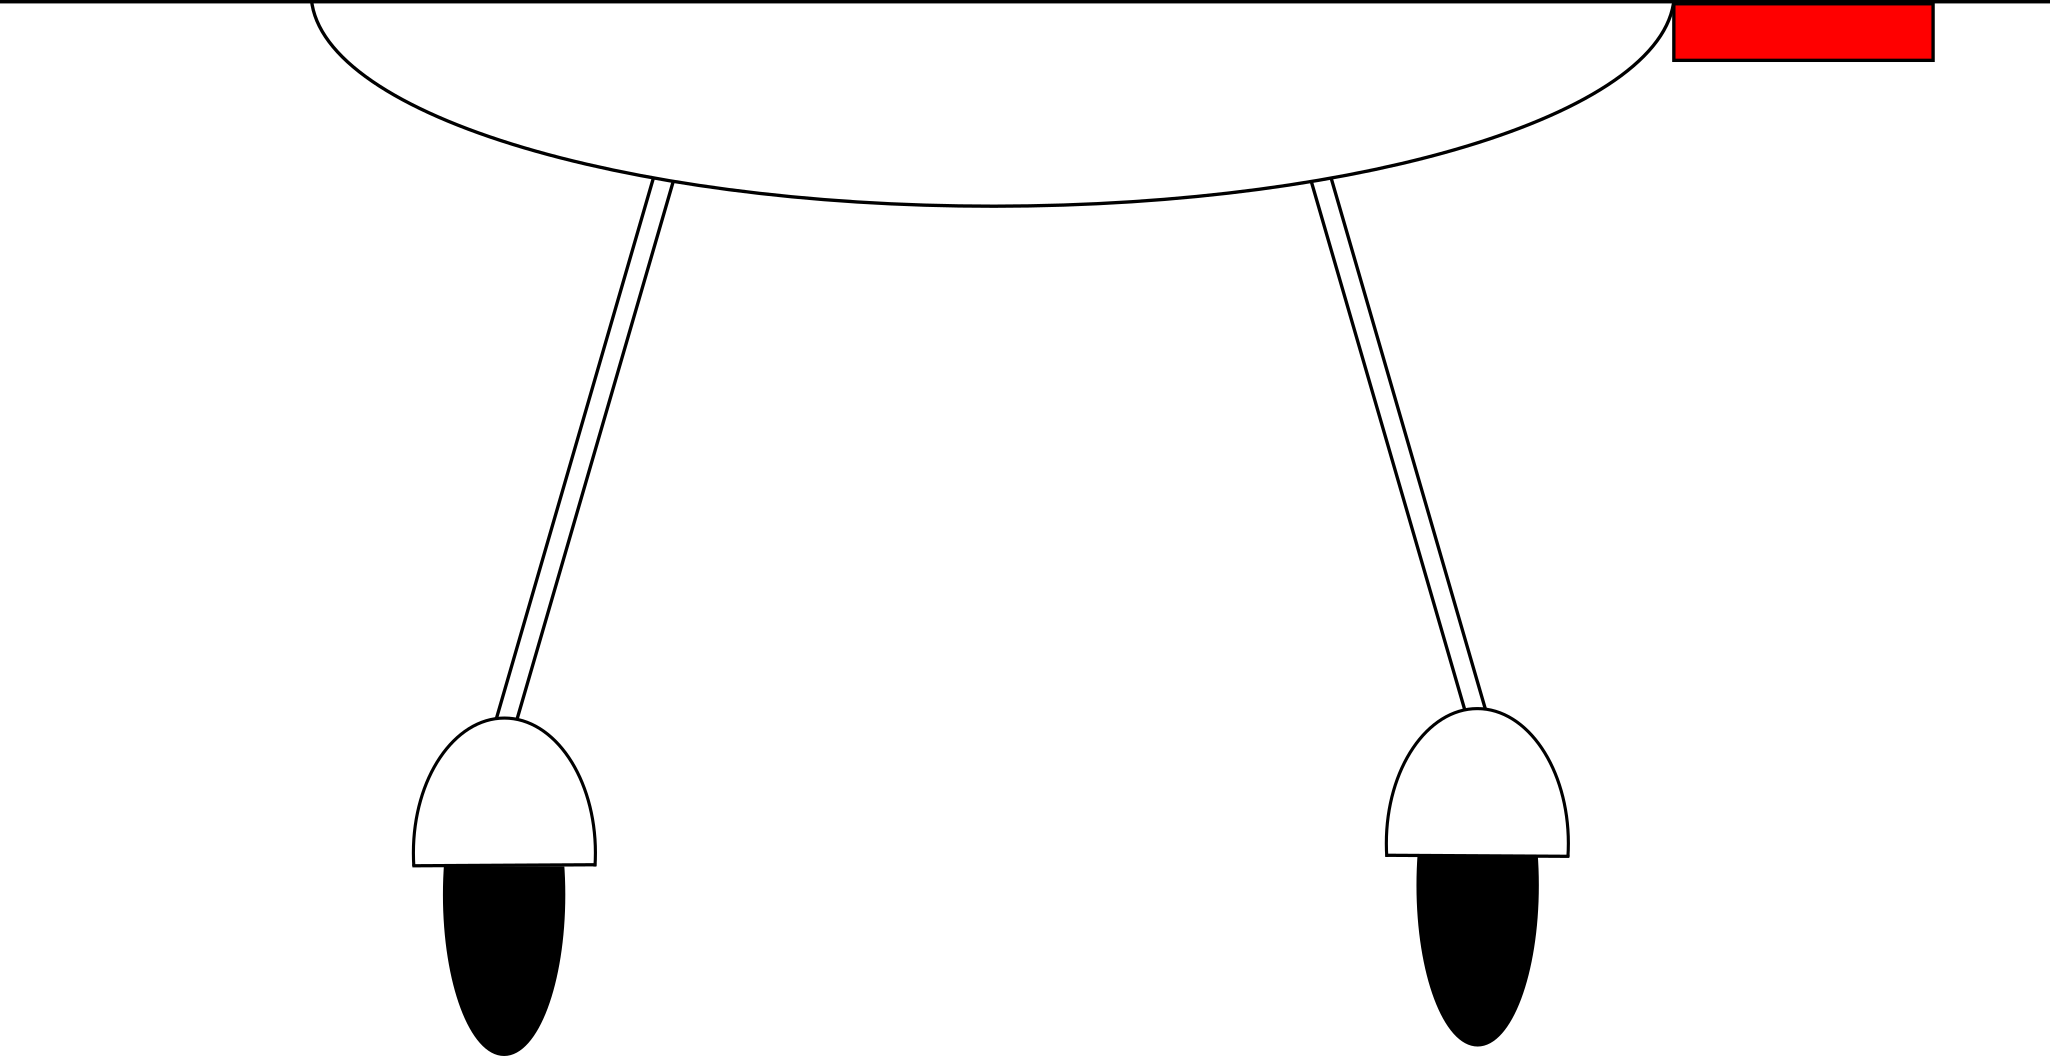
\includegraphics[scale=0.5]{obrazky-figures/umisteni_na_kridle.png}
					\caption{Montáž na spodní části křídla}
					\label{navrh::umisteni_kridlo}
				\end{center}
			\end{figure}
			
			\item na trup letadla, toto bohužel bude vyžadovat vrtání do trupu a~tudíž úpravu konstrukce letadla. Samozřejmostí pak musí být kalibrace modulu, stejně jako výše.
			
			\begin{figure}[H]
				\begin{center}
					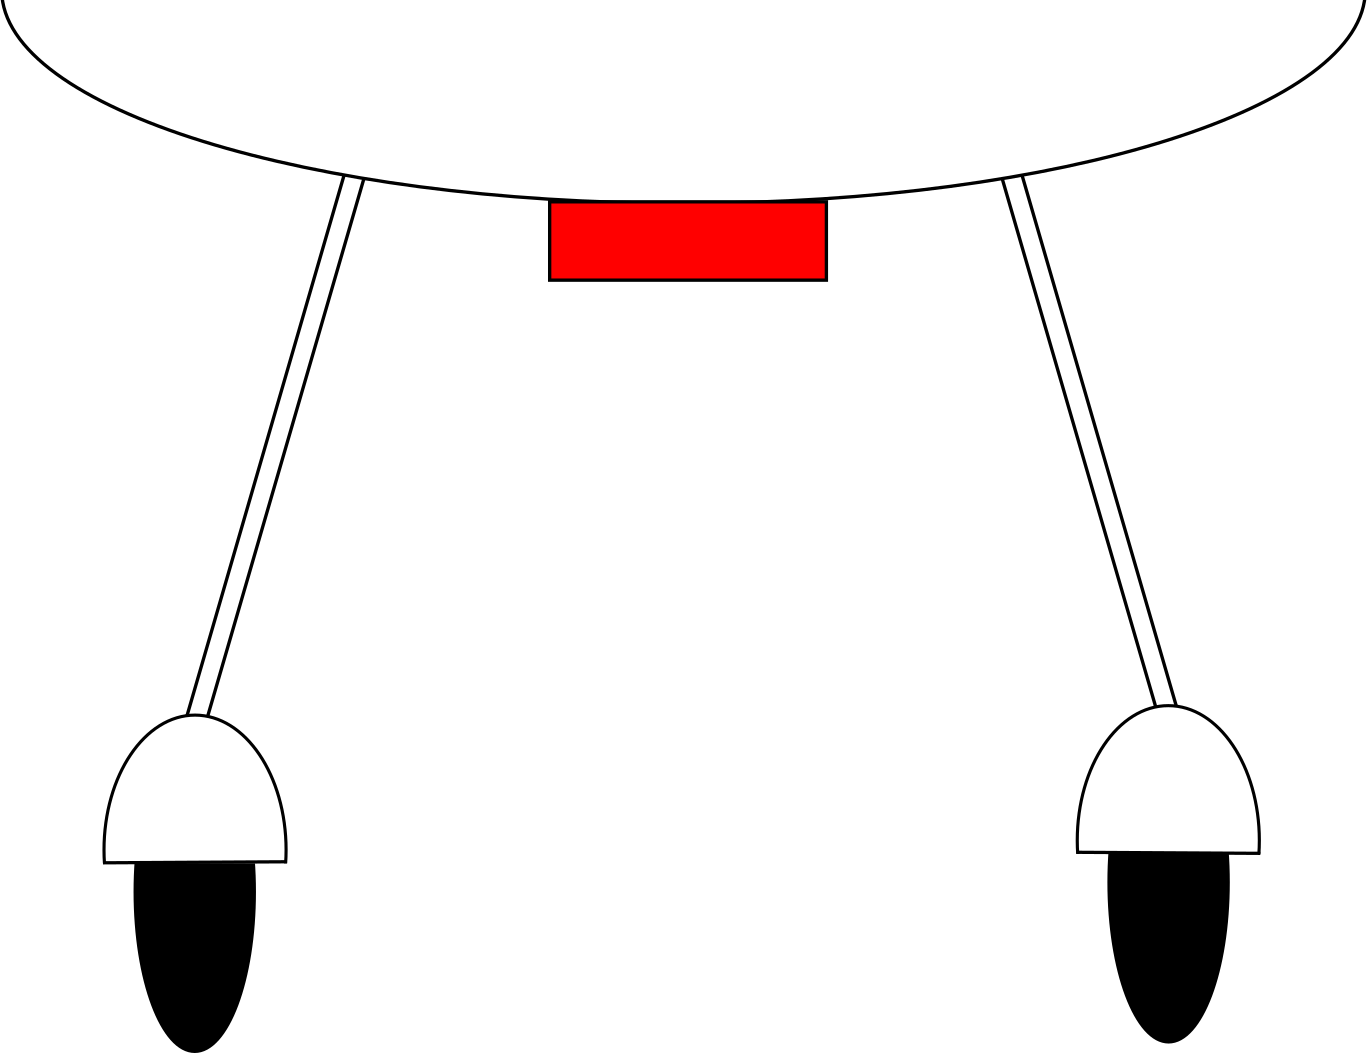
\includegraphics[scale=0.5]{obrazky-figures/umisteni_na_trup.png}
					\caption{Montáž na trup letadla}
					\label{navrh::umisteni_bricho}
				\end{center}
			\end{figure}
			
			\item do trupu letadla, ideálně do~odpružené schránky ať se zařízení nepoškodí. Zde je třeba vzít v úvahu materiál trupu letadla a jeho propustnost elektromagnetického záření případně. Zároveň je třeba zachovat možnost snadného přístupu k zařízení. S touto možností je třeba počítat již při návrhu letadla. Tudíž bude finančně nákladná.
			
			\begin{figure}[H]
				\begin{center}
					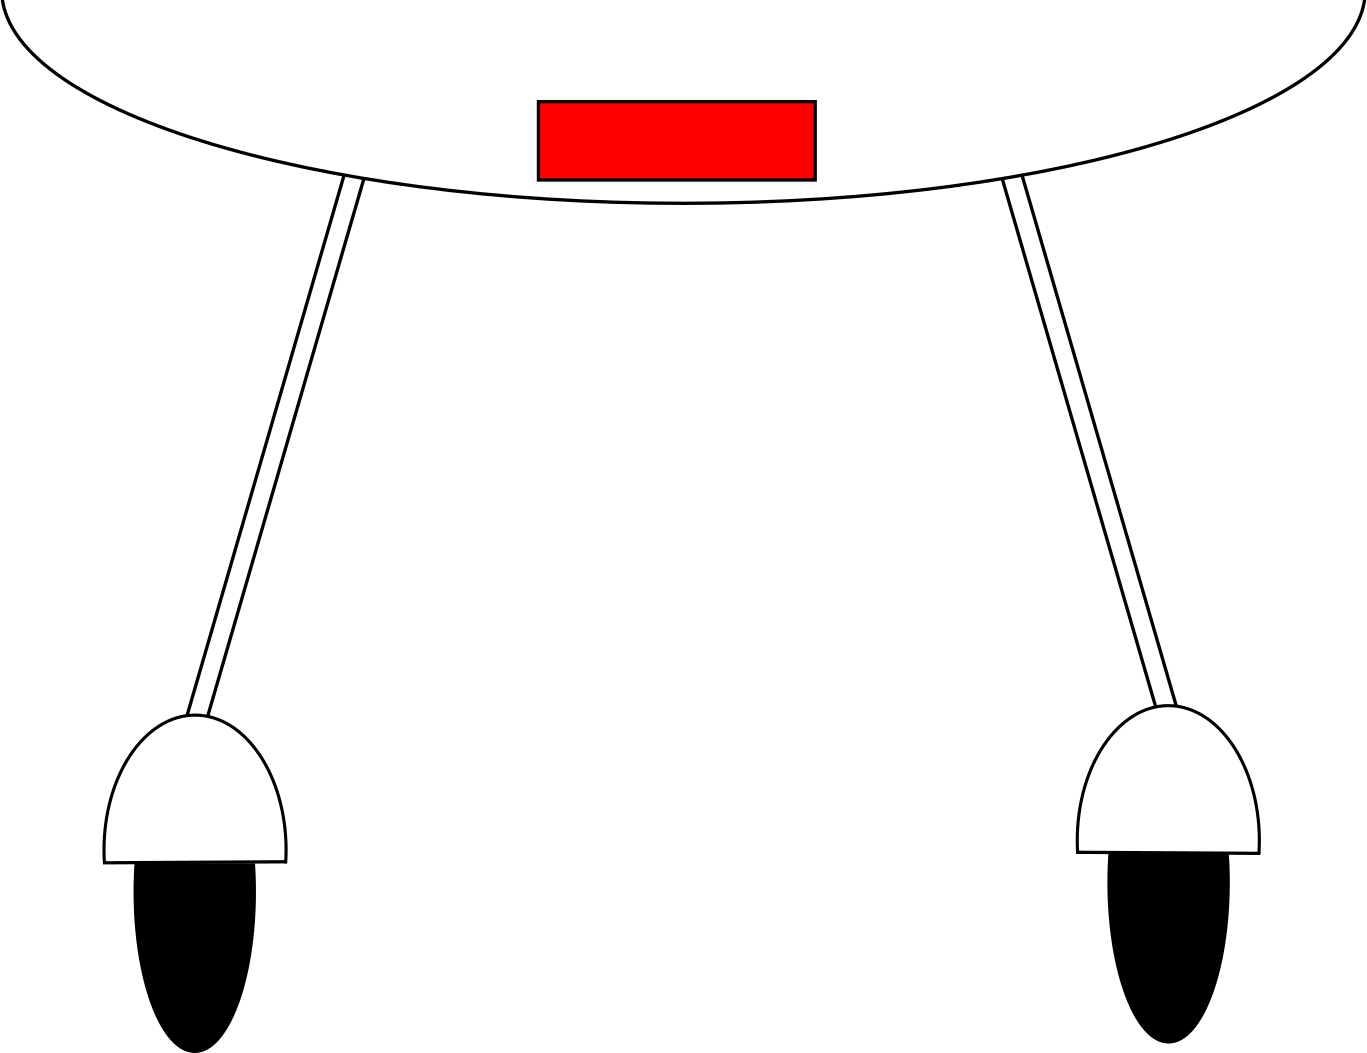
\includegraphics[scale=0.5]{obrazky-figures/umisteni_v_trupu.png}
					\caption{Montáž do trupu letadla}
					\label{navrh::umisteniuvnitr}
				\end{center}
			\end{figure}
			
		\end{itemize} 
		
		Pro testování bude vhodné uchycení na nohu s odsazením, jelikož bude vyžadovat nejmenší zásahy do konstrukce letadla, bude k zařízení snadný přístup a hlavně bude nejlevnější.
		Naopak pro produkční modely již bude vhodné zakomponovat tento výškoměr do letadla. To už záleží na zákazníkovi.
		
\chapter{Implementace}
	V předchozí kapitole jsme si pověděli co budeme dělat. Nyní si řekneme jak to budeme dělat, co k tomu budeme potřebovat a proč to tak budeme dělat.\par
	
	\section{Systémové prerekvizity}
	Abychom aplikaci vůbec spustili, musí na dodané platformě běžet operační systém. Mohli bychom dlouze polemizovat nad výhodami jednotlivých linuxových distrubucí, jestli vybrat binární nebo distribuovanou pomocí zdrojových kódů či vybrat podle balíčkovacího systému. Naštěstí toto nemusíme řešit, jelikož na cílové platformě je předinstalovaný operační systém OpenSUSE. Pro naše účely zcela postačuje.\par
	Jako další potřebujeme ovladač pro externí zvukovou kartu připojenou pomocí USB. Kvůli jednoduchosti a jednostrannosti použijeme ovladač ALSA. Ovšem aby ALSA detekovala externí zvukovou kartu, musí ji správně detekovat systém. Proto je důležité zavedení modulu snd-usb-audio do jádra operačního systému. Bez tohoto modulu jádro vidí externí zvukovou kartu pouze jako neznámé USB zařízení.\par
	
	\section{Jazyk}
	Abychom mohli vybrat konkrétní jazyk, musíme stanovit požadavky aplikace. Jak víme, každý jazyk má svá pro a proti.\par
	Můžeme vybírat z několika paradigmat a z nich odvíjejících se vlastností a míry abstrakce. Také se musíme rozhodnout, jestli chceme jazyk překládaný, či interpretovaný. V našem případě potřebujeme jazyk, který umožňuje psát programy, které nespotřebovávají příliš mnoho výpočetního výkonu, poskytuje vysokou míru abstrakce a zároveň umožňuje psát nízko běžící programy. Dále musí dobře odladěné knihovny a podporu komunity. Do tohoto rámce zapadá jen několik jazyků. Pro jazyk Java mluví jeho schopnost fungovat na mnoha platformách, vysoká úroveň abstrakce a relativně jednoduchý vývoj software v tomto jazyce. Bohužel, jeho největší přednost fungovat na mnoha platformách je v našem případě jeho největší nevýhodou. Platformu známe a virtuální stroj potřebný ke spouštění bajtkódu(bytecode) má příliš vysoké nároky na procesorový čas. Dalším vhodným kandidátem se zdá být Python. Ve prospěch Pythonu mluví možnost neuvěřitelně rychlého vývoje. Další výhodou je velké množství knihoven poskytující výbornou podporu pro vývoj. Proti mluví fakt, že se jedná o interpretovaný jazyk, který sice lze přeložit do C/C++, ale stále nedosahuje rychlostí C/C++. Jeho další nevýhodou je Global Interpreter Lock, který omezuje paralelní zpracování dat, nemluvě o jeho vysoké spotřebě paměti, protože všechno je objekt.\par
	Přikloňme se tedy k překládaným jazykům. Na první příčce rychlosti vykonávaného kódu sedí Assembler. Díky své nízké úrovni abstrakce a nízkoúrovňovému běhu poskytuje bezkonkurenční rychlost za předpokladu, že kód je správně napsán. Bohužel právě kvůli své nízké úrovni abstrakce je vývoj v tomto jazyce neúměrně náročný získanému výkonu. Další nevýhodou je jeho nepřenositelnost mezi platformami a v případě přechodu na novější verzi procesoru by se musely provést neúměrně velké zásahy do kódu.\par
	Přikloňme se tedy k tzv. vysokoúrovňovému Assembleru, jazyku C/C++. Pro jazyk C/C++ svědčí jejich relativně vysoká úroveň abstrakce, relativně rychlý vývoj za zachování nízkých hardwarových nároků a podpora v podobě mnoha knihoven, modulů a frameworků. Tento jazyk mimo jiné podporuje pohodlnou implementaci vícevláknového zpracování dat, které jsme si navrhli v předchozí kapitole.
	
	\section{Použité knihovny}
	Na naprostou většinu operací nám stačí knihovny, které již jsou obsaženy v systému. Dále ale potřebujeme knihovny, které nám umožní ovládat framework ALSA a s jeho pomocí generovat zvukový signál. V tomto konkrétním případě použijeme knihovnu PortAudio. PortAudio je multiplatformní otevřená knihovna pro vstupně/výstupní zvukové operace. Toto API poskytuje možnosti asynchronního volání funkcí a další nástroje pro generování zvukového signálu. Knihovna je implementována v jazyce C a je možno ji použít i v jazyce C++. Také na ní existuje nástavba v jazyce Python. Ten ale v této práci nevyužíváme.
	
	
	\section{Vícevláknová obsluha požadavků}
	Kvůli vícevláknové implementaci, kdy jedno vlákno zprávy přijímá a předává druhému, které na základě těchto zpráv generuje výstup, se musíme zamyslet nad zabezpečením mezivláknové komunikace.\par
	U přenosu dat mezi vlákny je důležité zachovat jejich konzistenci a zabránit nesynchronizovanému přístupu ke sdíleným zdrojům. V našem případě je tím zdrojem fronta sdílená mezi dvěma vlákny.\par
	Systém Linux poskytuje několik způsobů zabezpečení paralelních operací. Pro naše použití bude bohatě postačovat binární semafor mutex. Aby se autor nemusel zaobírat řešením synchronizace při vstupu do kritické sekce, implementoval si vlastní vláknově bezpečnou frontu(FIFO) a zásobník(FILO). Fronta a zásobník jsou implementovány pomocí šablonových tříd umístěných ve jmenném prostoru \texttt{threadSafety} v souboru \texttt{threadSafety.h}. Implementace pomocí šablon nám umožňuje vytvoření instancí pro jakékoliv jednoduché či složené datové typy a tím zaručuje obecnost použití. Rozhraní tříd je jednoduché a neobsahuje zbytečnosti. Vnitřní implementace tříd obsahuje frontu, do které ukládáme data, mutex, kterým zabezpečujeme kritickou sekci, \texttt{std::condition\_variable} pro detekci vložení prvku do fronty, atomický příznak(\texttt{std::atomic}) datového typu \texttt{bool} pro signalizaci prázdné fronty. Pro obsluhu mutexu se využívá vymoženost standardu C++11 \texttt{std::unique\_lock}, který při vytvoření v konstruktoru správně inicializuje a uzamkne mutex, a při zrušení proměnné daný mutex ve svém destruktoru správně uvolní. Mezi frontou a zásobníkem jsou dva rozdíly. Prvním rozdílem je využití fronty s dvojitým koncem pro implementaci zásobníku a druhým je modifikace rozhraní nahrazením veřejné položky \texttt{T \&front()} položkou \texttt{T \&top()}. Z pohledu uživatele těchto tříd je jejich chování stejné. Obě položky vrací referenci na prvek, který bude po zavolání metody \texttt{T pop()} z objektu vyjmut jako první a bude zkopírován do uživatelem zvolené proměnné.\par
	Po zajištění konzistence přístupu ke sdílenému zdroji musíme zajistit zpracování pouze aktuálních informací. Toto je zajištěno tříděním zpráv podle časového razítka přijímaného z modulu zpracovávající radarová data. Komunikační modul si vygeneruje své časové razítko, porovná jej s přijatým razítkem a za předpokladu, že je v povoleném limitu 150 milisekund generuje zvuk. V případě, že není, je zpráva zahozena a na řadu přichází aktuálnější.
 	
	\section{Princip generování zvuku}
	Zvuk je generován pomocí API poskytovaným knihovnou PortAudio. Nejdříve si povíme o obecném principu fungování tohoto API a následně se zaměříme na konkrétní implementaci v této práci.\par
	Nejdříve musí dojít i inicializaci. Pro to potřebujeme získat informace o výstupních zařízeních a otevřít zvukový kanál. Při otevírání dáváme API k dispozici adresu statické funkce, která bude asynchronně volána během běhu programu(callback). Tato funkce generuje signál, který je dále posílán do ALSA API. Programátor tak je odstíněn od nízkoúrovňového programování. Komunikace mezi programátorem callbackem probíhá pomocí statické struktury definované jako globální proměnná. Jelikož je globální, hodnoty ve struktuře jsou překladačem inicializovány na nuly. Díky tomu program začíná generovat zvuk až po nastavení frekvence ve vlákně generující výstup.\par
	Nyní nám vyvstává problém generování správné ho signálu. Po kontrole konzistence přijatých dat generujeme obdélníkový signál. Zvukový signál musí indikovat vertikální přibližování k dráze a tudíž se pauza mezi tóny a délka tónu musí vhodně zkracovat. Musíme také počítat s konfigurací, kdy každé letadlo má výšku výdrže jinou. Z toho důvodu musíme použít vhodný vztah pro výpočet. Experimentálně bylo zjištěno, že výraz: \[\texttt{25000~/~(výška~výdrže[m])}\] je vhodný pro výšky výdrže pod 3~metry a nad tři metry je vhodný výraz níže. \[\texttt{25000~/~(výška~výdrže[m]~/~2)}\]
	Tento výraz je využit jako koeficient pro násobení výšky nad letištěm pro generování pauzy mezi tóny. Výsledek je v milisekundách.
	
	\section{Konfigurace a spuštění}
	Konfigurace probíhá modifikací přečtením konfiguračního souboru \texttt{/opt/cfg/radar.conf}. (zde prosím vedoucího o kontrolu)Spuštění se provádí vypínačem, kdy najede operační systém a ihned po jeho spuštění dojde ke spuštění programu simulující přistání a programu generující zvuk.
	TODO po konzultaci
	
	\section{Testování}
	Pro testovací účely komunikace mezi jednotlivými moduly a pro testování správného generování zvuku autor napsal testovací program, který do komunikačního protokolu iterativně vyplňuje všechny potřebné informace. Program využívá BSD schránek a odesílá UDP pakety dále.
	V reálných podmínkách bohužel nebylo možno systém otestovat, jelikož nám nebyl dodán původně domluvený algoritmus pro zpracování radarového signálu. 
	
\chapter{Závěr}
	V úvodu této práce jsme si vytyčili jisté cíle. Čtenář se seznámil se stručnou historií měření výšky a byl relativně detailně uveden do této problematiky. Vysvětlili jsme si významy pojmů QHN, AMSL a transition level. Dále byla čtenáři vysvětlena nepřesnost barometrických výškoměrů, tzv. aneroidů, tato nepřesnost byla zdůvodněna a čtenáři bylo vysvětleno, proč chyba měření výšky pomocí aneroidu nezpůsobí srážku letadel ve vzduchu.\par
	Čtenáři také byl stručně přiblížen vývoj radaru a byly popsány použité technologie v našem řešení. Následně byl čtenář uveden do problematiky řízení letového provozu, konkrétně fáze přistání, jak se dělí a jaké nástrahy v jednotlivých fázích může pilot očekávat.\par
	Naším hlavním cílem ovšem byl návrh systému, který by usnadnil výuku přistání začínajícím pilotům a zvýšil její bezpečnost. V této kapitole jsme se zamysleli nad vhodnými platformami pro toto konkrétní použití jak z hlediska operačního systému tak z hlediska použitelných procesorů. Dále jsme se zamysleli nad podobou vstupního a výstupního hardware s analýzou dopadů na pozornost pilota, důrazem na jednoduchost, efektivnost ovládaní a přenosu informace pilotovi. Následně jsme si ukázali návrh komunikace mezi jednotlivými částmi se stručnou analýzou možných technologií pro implementaci komunikace. V té stejné sekci jsme si navrhli možnou architekturu programů běžících v našem systému. Po vyřešení této problematiky s důrazem na aktuálnost dat a tudíž bezpečnost posádky jsme si popsali komunikační protokol a zdůvodnili přítomnost jednotlivých položek. Na konci této kapitoly jsme se zamysleli nad umístěním hardware na letadle z několika pohledů ať to je testování či výsledná produkce.\par
	Po návrhu celého systému jsme přikročili k řešení implementace. Nejdříve jsme si vyjmenovali potřebné systémové prerekvizity pro zajištění správné funkcionality programového vybavení. Dále jsme se analyzovali vhodnost jednotlivých jazyků pro implementaci programového vybavení v našem zařízení. Samozřejmostí je výběr vhodných knihoven pro implementaci programového vybavení a zdůvodnění daného výběru. Řekli jsme si jak vypadá implementace vláknově bezpečné fronty pomocí šablon pro zjednodušení implementace a zobecnění použití. Taky jsme si ukázali kontrolu aktuálnosti přijatých dat ke zpracování. Následně jsme si vysvětlili princip generování zvuku s pomocí zvolené knihovny a její ovládání. Samozřejmostí je i popis konfigurace zařízení pro různé modely letadel, spuštění systému a na závěr jsme si vysvětlili postup testování systému.
	
	\section{Možné pokračování práce}
	
	
%=========================================================================
